\section{2D simulations}
In the first place we carried out 2D simulations in order to get a global view on the whole range of parameters.
Indeed, since the 3D case is exactly the same from a numerical point of view, we preferred to validate the numerical methods on a 2D set up first. 
For this study we considered a set of data made of $\sim 150$ simulations. 
The numerical parameters to carry out these simulations have been validated through other simulations that are not presented in this report. 
We used the following parameters $N = 10$ or  $N_b = 100$ and $L = 30 \delta$ for respectively, the number of bubbles and the mesh definition. 
Here is the range that we covered with the these parametric simulations, 
\begin{multicols}{2}
    \begin{itemize}
        \item $\rho_r = 1.66$,
        \item $0.01 \leq  \mu_r \leq 0.42$,
        \item $0.1  \leq  Bo    \leq 1$,
    \end{itemize}
    \begin{itemize}
        \item $0.05 \leq  \phi  \leq 0.25$.
        \item $0.1 \leq  Ga  \leq 100$.
    \end{itemize}
\end{multicols}
Note that we did not change the value of $\rho_r$ yet, so it is a fixed parameter in all our studies.
Obviously this dependency might need to be investigated in a future work.


\subsubsection*{Computation of the particles volume.}
\tb{numerical method}
The particle mass or volume, since $\rho_d$ is constant, is defined as, 
\begin{equation}
    m_\alpha 
    = \int_{V_\alpha} \rho_d dV.
\end{equation}
 On the code, Basilisk we discretize this expression by taking the following weighted sum,
\begin{equation}
    m_\alpha = \rho_d\sum_{i} V_i \chi_i \;\;\; \text{with} \;\;\;y_i \in V_\alpha,
\end{equation}
where, $\chi_i$ is the value of the color function at $y_i$ and $V_i$ the volume of the cell.
\subsubsection*{Computation of the particles averaged velocity.}
In this section we focus on the Computation of the mean velocity of the particles i.e. $\bm{u_\alpha}$. 
This point seems trivial at first, nevertheless, diving into the details can bring the answers of the questions asked \ref{chap:avg}, as well as validate or not the linear deformation assumption. 
We recall the expression of the momentum for a particle $\alpha$ :
\begin{equation}
    \bm{p}_\alpha 
    = \int_{V_\alpha} \rho_d \bm{u} dV
    = m_\alpha \bm{u}_\alpha 
    + \int_{V_\alpha} \rho_d \bm{w}_\alpha dV
    % \bm{P}_\alpha = \int_{V_\alpha} \rho_d \bm{w}_\alpha\bm{r}_\alpha dV.
\end{equation}
where $\bm{u}_\alpha$, is the velocity at the center of the particle $\alpha$ (different from the mean velocity of the particle $\alpha$). 
Note that this expression isn't directly invertible for $\bm{u}_\alpha$. 
Indeed, remark that $\bm{w}_\alpha$ is function of $\bm{u}_\alpha$.
Therefore, the quantity that is directly measurable on \texttt{basilisk} is $\bm{p}_\alpha$ not $\bm{u}_\alpha$. 
Indeed, it is important to understand that the velocity $\bm{u}_\alpha$ cannot be measured from the exact value of $\bm{p}_\alpha$.
In \ref{ap:cinematic} we decompose the velocity into its expansion along $\bm{y}_\alpha$. 
At the first order it yields, 
\begin{equation}
    \bm{p}_\alpha^l 
    = m_\alpha \bm{u}_\alpha + \mathcal{O}(\bm{r}_\alpha^2)
\end{equation}
where the superscript $^l$ stand for linear. 
In this situation we can recover the exact velocity of the particle from its momentum. 
On Basilisk, it is possible to compute the exact value of $\bm{p}_\alpha$ and the first order approximation of it by taking the velocity at the center of the particle. 
Therefore, the velocity fluctuation reads as, 
\begin{equation}
    \rho_d \int_{V_\alpha} \bm{w}_\alpha dV
    = \bm{p}_\alpha -\bm{p}_\alpha^l
    \approx \mathcal{O}(\bm{r}_\alpha^2)
\end{equation}
In practice we discretize this expression the same way as the mass calculation.
It yields, 
\begin{equation}
    \bm{p}_\alpha = \rho_d\sum_{i} V_i u_i \chi_i \;\;\; \text{with} \;\;\;y_i \in V_\alpha,
\end{equation}
\ref{fig:velfluc} shows that the fluctuation along the vertical axis scale as $~15\%$ of the total momentum, while the fluctuation around the horizontal axis is in average, null.
Besides, when $\mu_r \rightarrow 0$ and $Ga \rightarrow 0$ the relative fluctuation becomes negligible. 
Consequently, the fluctuations in the vertical direction are probably not negligible in the limit of high $Ga$ and $\mu_r$ in \ref{eq:particlesAVG}. 
\begin{figure}[h!]
    \centering
    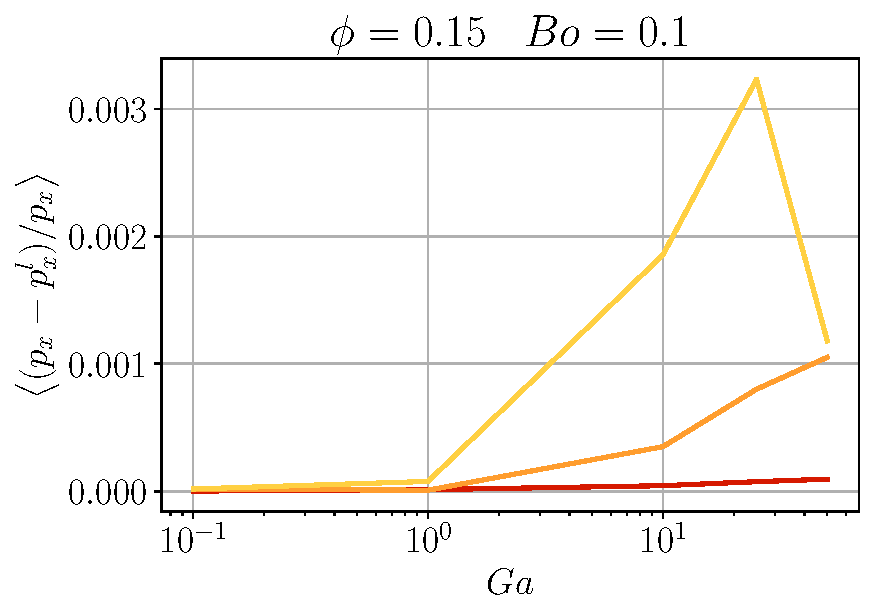
\includegraphics[height = 0.3 \textwidth]{image/LINEAR/pl/x_Bo_0_1_PHI_0_15.pdf}
    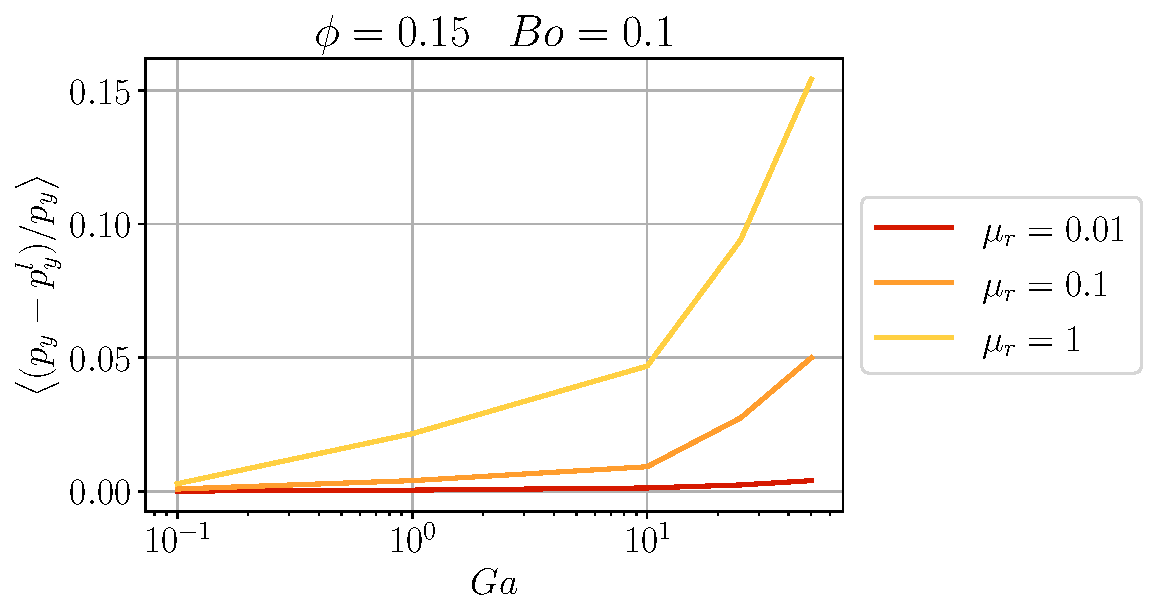
\includegraphics[height = 0.3 \textwidth]{image/LINEAR/pl/y_Bo_0_1_PHI_0_15.pdf}
    \caption{Averaged momentum fluctuation on the vertical and horizontal axis.}
    \label{fig:velfluc}
\end{figure}
Besides, the fact that there is fluctuation prove that the motion inside the particles are not linear (which is what we could expect from droplets ).
\tb{Need to change the graphs and add the dependency with $Bo$}

\tb{\subsubsection*{Computation of the particles averaged rate of strain and rotation.}}
Next, we compute the averaged moment of momentum. 
We can compute the exact value of the moment of momentum, namely, 
\begin{equation}
    \bm{P}_\alpha 
    = \int_{V_\alpha} \rho_d \bm{r}_\alpha\bm{u}_\alpha dV.
\end{equation}
or,
\begin{equation}
    \bm{P}_{\alpha} 
    =\sum_{i}  \bm{u}_{i}\bm{y''}_{i} dV_i
    \;\;\; \text{with } y_i \in V_\alpha
\end{equation}
% \begin{equation}
%     \bm{C}_{\alpha} 
%     =\int_{V_\alpha} \rho_d \bm{u}_\alpha\bm{r}_\alpha dV \cdot\bm{\mathcal{G}_\alpha}^{-1}
%     =\int_{V_\alpha} \rho_d \bm{u}_\alpha\bm{r}_\alpha dV \cdot\left(\int_{V_\alpha} \rho_d\bm{r}_\alphadV\right)^{-1}
% \end{equation}
Similarly, we can not recover the exact value of the angular velocity nor the value of the rate of strain.
Nevertheless, if we consider only first order displacement (see \ref{ap:cinematic}), it yields, 
\begin{equation}
    \bm{P_\alpha}
    = \bm{\mathcal{G}_\alpha}  \cdot \bm{\epsilon} \cdot \bm{\omega_\alpha} 
    + \bm{\mathcal{G}_\alpha} \cdot \bm{E_\alpha}. 
\end{equation}
Taking the symmetric part and antisymmetric part of this equation provide one equation for the rate of strain and another for the angular velocities. 
Thus, at the first order we can consider the following relation, 
\begin{equation}
    \bm{\epsilon} \cdot \bm{\omega_\alpha}
    = \frac{1}{2}(\bm{P}_\alpha - \bm{P}_\alpha^T) \cdot\bm{\mathcal{G}}_\alpha^{-1}
    \;\;\;
    \bm{E}_\alpha
    =(\bm{P}_\alpha + \bm{P}_\alpha^T)  \cdot\bm{\mathcal{G}}_\alpha^{-1}
\end{equation}
Also from the conservation of momentum we know that, 
\begin{equation}
    \bm{\omega_\alpha}
    = \bm{\mathcal{I}}_\alpha^{-1} \cdot \rho_d \int_{V_\alpha}\bm{u}_\alpha \times\bm{r}_\alpha dV 
\end{equation}
which can be rewritten as, 
\begin{align*}
    \bm{\omega_\alpha}
    &=  \bm{\mathcal{I}}_\alpha^{-1}\cdot\epsilon : \bm{P}_\alpha \\
    \bm{\omega_\alpha}
    &=  \bm{\mathcal{I}}_\alpha^{-1} \cdot \epsilon : \bm{P}_\alpha 
\end{align*}

\subsubsection{Computation of the hydrodynamical first moment}

In order to compute $\bm{M}^h_\alpha$ on each droplet we used the volume integral formulation.
Indeed, the first moment reads as,
\begin{align}
    (M^h_\alpha)_{ij}
    & = \int_{S_\alpha} r_i \sigma_{jk} n_k dS \\
    & = \int_{V_\alpha} \partial_k \left( r_i \sigma_{jk} \right) dV \\
    &= \int_{V_\alpha} \sigma_{ji}  dV
    + \mu_d \int_{V_\alpha} r_i \partial_k\sigma_{jk} dV
\end{align}
using $\sigma_{ij} = -p\delta_{ij} + \mu \left(\partial_j u_i + \partial_i u_j\right)$ we get, 
\begin{equation}
    (M^h_\alpha)_{ij}
    = - \int_{V_\alpha} p\delta_{ji}  dV
    +  \mu_d\int_{V_\alpha} \left(\partial_i u_j+\partial_j u_i\right)dV
    - \int_{V_\alpha} r_i \partial_j p \;dV,
    + \mu_d \int_{V_\alpha} r_i \partial_k\partial_k u_j dV
\end{equation} 

\subsubsection{Drag force term}
The relative vertical velocity of the droplets with respect to the mean fluid motion, referred as $U$, becomes constant after a certain amount of time $t_{min}$.
Besides, we know that all the droplets experience a force of magnitude $\bm{F} = \phi \mathcal{L}^2 \Delta \rho \bm{g}$, where $\mathcal{L}$ is the domain size.
Thus, the averaged drag force per droplets is simply :
\begin{equation}
    \frac{\left<\bm{f}_\alpha\right>}{\mu_f UD} = \left<V_b\right>\frac{\bm{g}\Delta \rho }{\mu_f D U}
    \label{eq:avgF}
\end{equation}  
where, $V_b$ is the averaged volume of droplets. 
We recall that the following results are carried out for a uniform distribution of bubbles thus $V_b = \left<V_b\right>$.
Besides, \ref{eq:avgF} is non-zero only on the vertical axis since $\bm{g} = g \bm{e}_y$. 
The drift velocity is computed by averaging the relative velocity on the time range where it is statistically stable.
This time range goes from $t = t_{min}$ to $t = t_{max}$, where the value of the dimensionless times are $t_{min} = 250$ and $t_{end} = 1000$. 
Thus, if we note $\left<\bm{u}_\alpha\right>^p(t)$ the instantaneous averaged velocity of the dispersed phase and $\left<\bm{u}\right>^f(t)$ the velocity of the fluid phase,
\begin{equation}
    \bm{U} =\left(t_{min}-t_{end}\right)^{-1}\int_{t_{min}}^{t_{end}}\left[\left<\bm{u}\right>^d(t)-\left<\bm{u}\right>^f(t)\right] dt.
\end{equation}

On the left graphic, \ref{fig:avgF}(left), we can note that the \textit{Bond number} has no influence on the mean drift velocity $\bm{U}$ for the set of parameters considered.
Indeed, as said in introduction, we are interested in very low \textit{Bond number} (see \ref{tab:parameters}).
Since there is no variation in the range $Bo = [0.1,1]$, we can consider that the system has reached its asymptotic behavior at $Bo<1$.
Furthermore, we also noted almost no variation with $Bo$ for all the other sets of parameters.
Consequently, the \textit{Bond number} dependency won't be considered in the present section. 
\begin{figure}[h!]
    \centering
    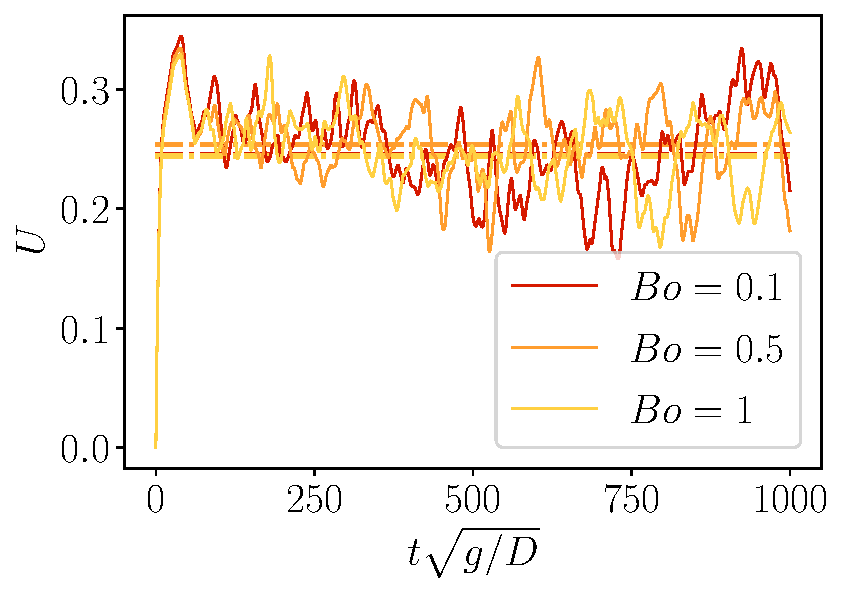
\includegraphics[height=0.22\textheight]{image/N_10/Favg/Bosdep_Ga_50.pdf}
    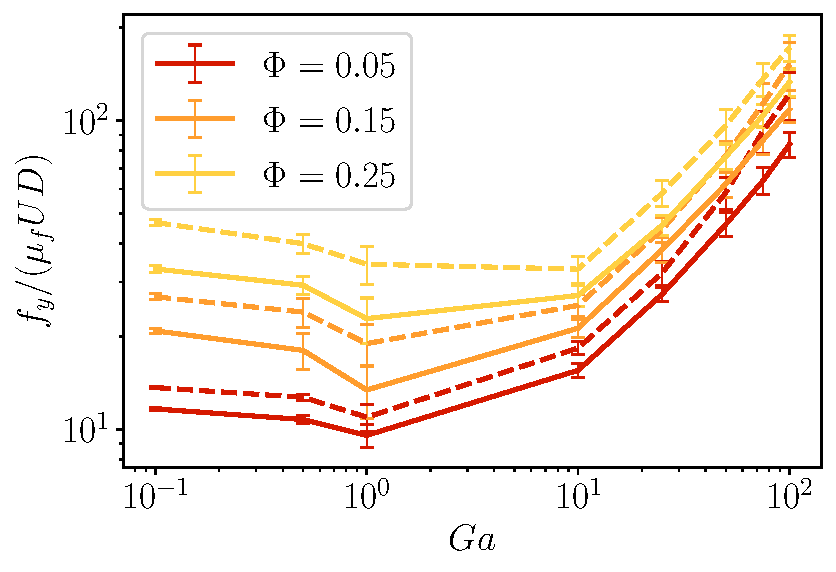
\includegraphics[height=0.22\textheight]{image/N_10/Favg/F_mu_Bo_0_5.pdf}
    \caption{(left) : Relative velocity in terms of the dimensionless time for different $Bo$ for $\phi = 0.15$, $\mu_r = 0.042$ and $Ga = 50$. (right) : Averaged drag force per droplets. Dashed lines : $\mu_f = 0.42$, solid lines : $\mu_f = 0.042$. The results are shown for $Bo = 0.5$.} 
    \label{fig:avgF}
\end{figure}
On the right graphic of \ref{fig:avgF} we can observe that for some studies at $Ga\le 1$, the dimensionless force is independent of the  \textit{Galileo number}. 
Besides, the averaged drag force increase with the volume fraction of droplets $\phi$.
While it decreases with increasing $\mu_r$. 

In the objective of designing the empirical formula describing the averaged force, we consider two steps. 
In the first place we consider a function, $g(\phi,\mu_r)$, independent of $Ga$ and $Bo$, which is asymptotic to $\bm{f}$ in the law $Ga$.
Then, the averaged force must be expressed by, $\bm{f} = \bm{g} \left[g(\phi,\mu_r) + f(\phi,\mu_r,Ga)\right]$ with $f(\phi,\mu_r,Ga)$ vanishing for small $Ga$. 
Besides, for $\phi \rightarrow 0$, the averaged force must tend to the isolated case scenario noted $\bm{f}_i(\mu_r)$. 
When $\phi \rightarrow 1$ the drag force must tend to infinity since no fluid goes through. 
Similarly, at $\mu_r \rightarrow \infty$, $\bm{f}_i$ must tend to the rigid spheres drag forces case,
at $Ga \rightarrow 0$ this force is comparable to the stokes drag force, referred as $\bm{f}_s$ \citep{guazzelli2011} ($\bm{f}_s/(\mu_r U D) = 3\pi$ for spheres, and \cite{khayat1989inertia}). 
And, when $\mu_r \rightarrow 0$ we should recover the drag force on rising bubbles from \citet{tomiyama1998drag}, we will note this force $\bm{f}_b$. 
Therefore, the function $g$ must respect the following composition,
\begin{equation}
    g(\phi,\mu_r) = \frac{C_1}{\phi - 1} + (\bm{f_i} - \bm{f_b}) e^{-\mu_r} + \bm{f_b}
\end{equation}
As one can observe on \ref{fig:avgF} the dependency with $Ga$, when $Ga>10$, behave as a power law. 
Therefore, 
\begin{equation}
    f(\phi,\mu_r,Ga) = C_1 Ga^{C_2}
\end{equation}

\subsubsection{Pseudo turbulence}
The averaged equations for fluid and particulate phase seen \ref{chap:avg} need two-Pseudo turbulent tensor correlation,
namely, $\left<\bm{u'u'}\right>^p$ and $\left<\bm{u'u'}\right>^f$. 
Those tensors can be calculated as it is in the CFD code, since it is only fields variable average. 
Also, since our domain is periodic the crossed terms should be equal to 0.
Let's start by evaluating the fluid-phase average velocity fluctuations.
First note, that in the averaged equations, the important term isn't the pseudo-turbulent tensor itself but its divergence, namely,
\begin{equation*}    
    \left(\bm{\nabla} \cdot \left<\bm{u}'\bm{u}'\right>^f \right)_j = \frac{\partial <u_i' u_j'>^f}{\partial x_i}
\end{equation*}
where we make use of Einstein summation notation.
If the diagonal components are indeed null, it yields,
\begin{equation*}    
    \left(\bm{\nabla} \cdot \left<\bm{u}'\bm{u}'\right>^f \right)_j 
    = \frac{\partial <u_j' u_j'>^f}{\partial x_j}
\end{equation*}
\begin{figure}[h!]
    \centering
    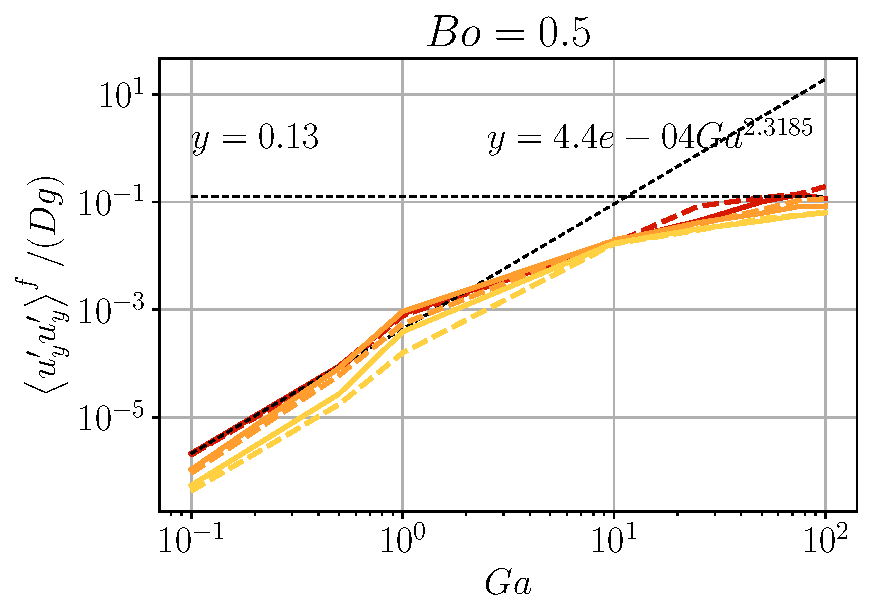
\includegraphics[height=0.20\textheight]{image/N_10/UU/UU_fyy_Bo_0_5.pdf}
    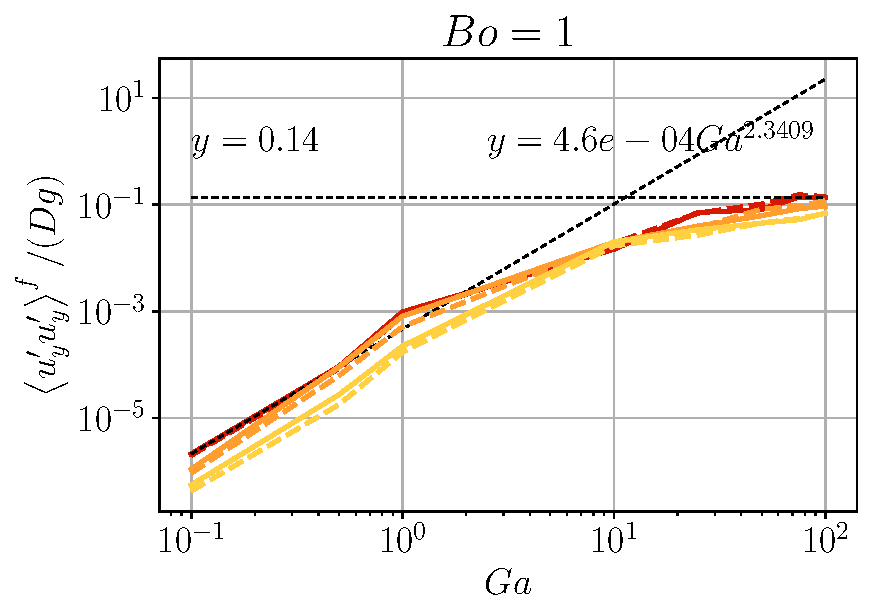
\includegraphics[height=0.20\textheight]{image/N_10/UU/UU_fyy_Bo_1.pdf}
    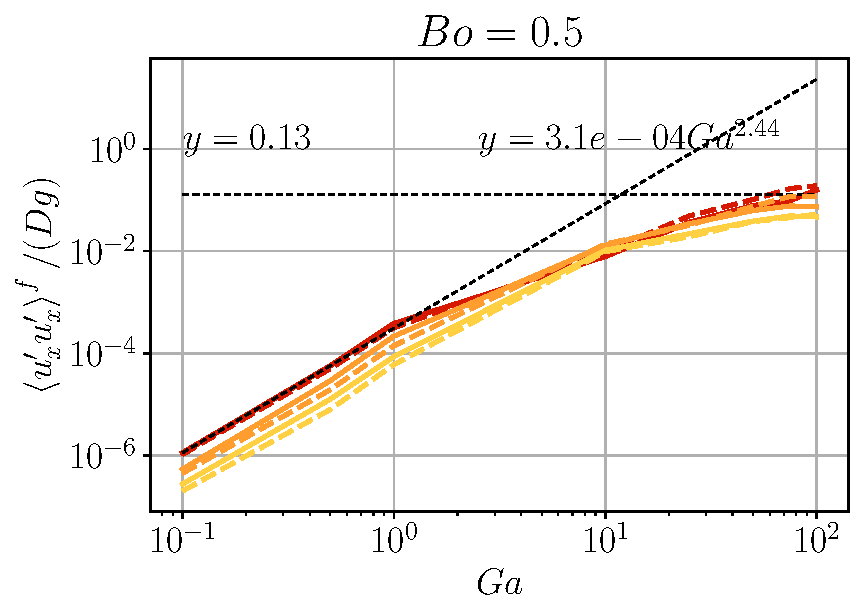
\includegraphics[height=0.20\textheight]{image/N_10/UU/UU_fxx_Bo_0_5.pdf}
    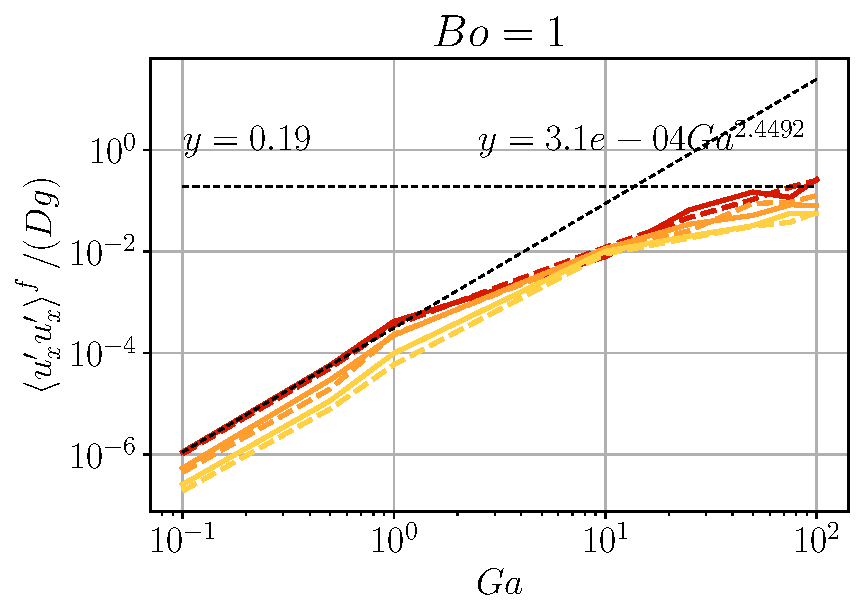
\includegraphics[height=0.20\textheight]{image/N_10/UU/UU_fxx_Bo_1.pdf}
    \caption{Fluid-phase average of the dimensionless velocity fluctuations. Dashed lines : $\mu_f = 0.42$, solid lines : $\mu_f = 0.042$, Dotted lines : asymptotic fit for $\phi = 0.05$ and $\mu_r = 0.42$. The color stand  \textcolor{red}{\textbf{--}} : $\phi = 0.05$, \textcolor{orange}{\textbf{--}} : $\phi = 0.15$, \textcolor{yellow}{\textbf{--}} : $\phi = 0.25$} 
    \label{fig:UUf}
\end{figure} 
On \ref{fig:UUf} we can observe that the diagonal of the pseudo-turbulent tensor $\left<\bm{u'u'}\right>^f$ weakly dependent on $\mu_r$ nor on $\phi$.
Regarding the dependency of  with $Ga$, we note a power law behavior when, $Ga \rightarrow 0$. 
We can note that $\left<{u_x'u_x'}\right>^f  < \left<{u_y'u_y'}\right>^f$ for low $Ga$.
Indeed, the fluctuation in the $\bm{e}_y$ direction are more important due to the gravity along this axis.  
Nevertheless, it is not necessarily true for the large $Ga$. 
\ref{fig:UUp} shows the particulate-phase average exhibit the same behavior as the fluid phase average. 
Nevertheless, the $x$ and $y$ fluctuation have the same value.
\begin{figure}[h!]
    \centering
    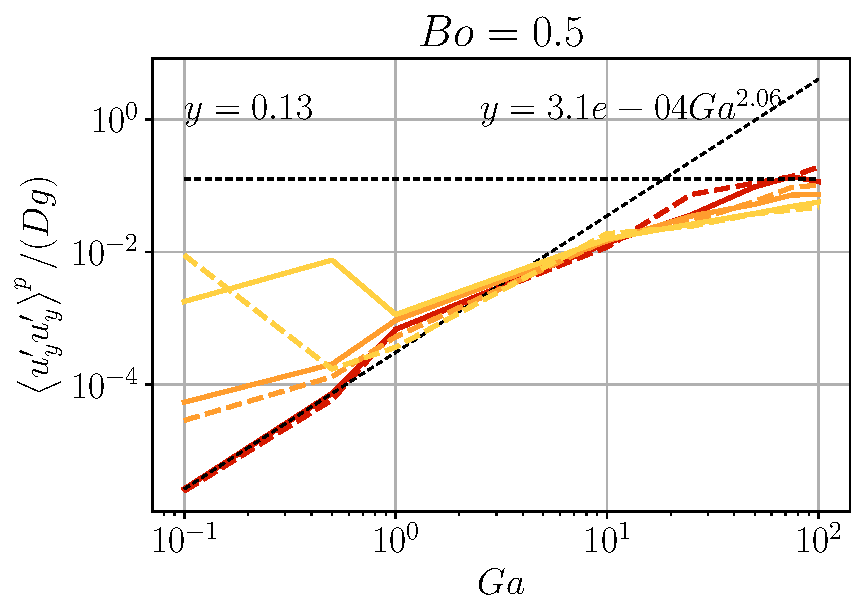
\includegraphics[height=0.20\textheight]{image/N_10/UU/UU_pyy_Bo_0_5.pdf}
    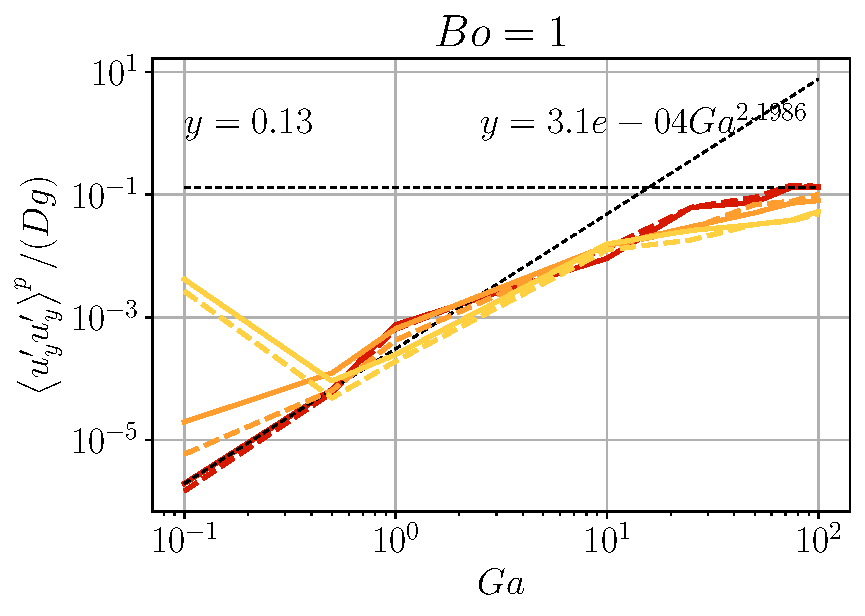
\includegraphics[height=0.20\textheight]{image/N_10/UU/UU_pyy_Bo_1.pdf}
    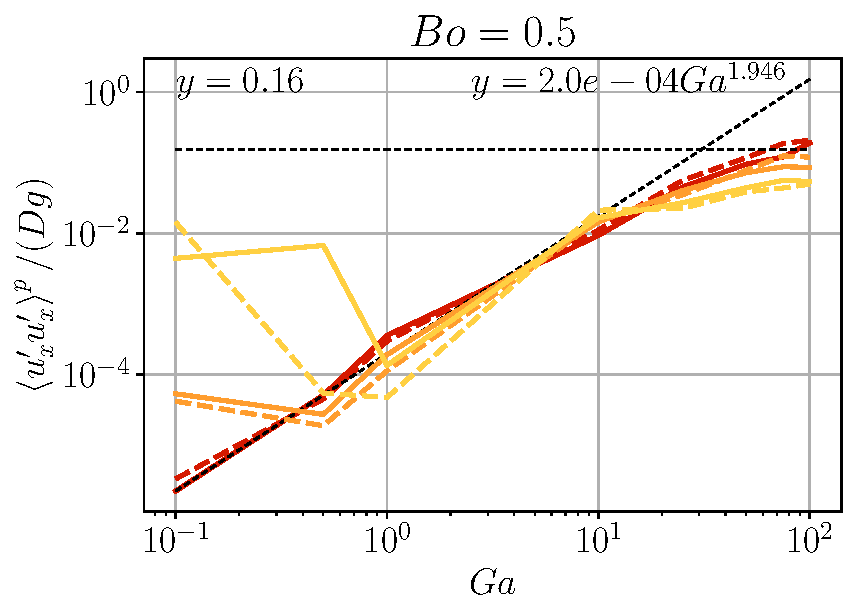
\includegraphics[height=0.20\textheight]{image/N_10/UU/UU_pxx_Bo_0_5.pdf}
    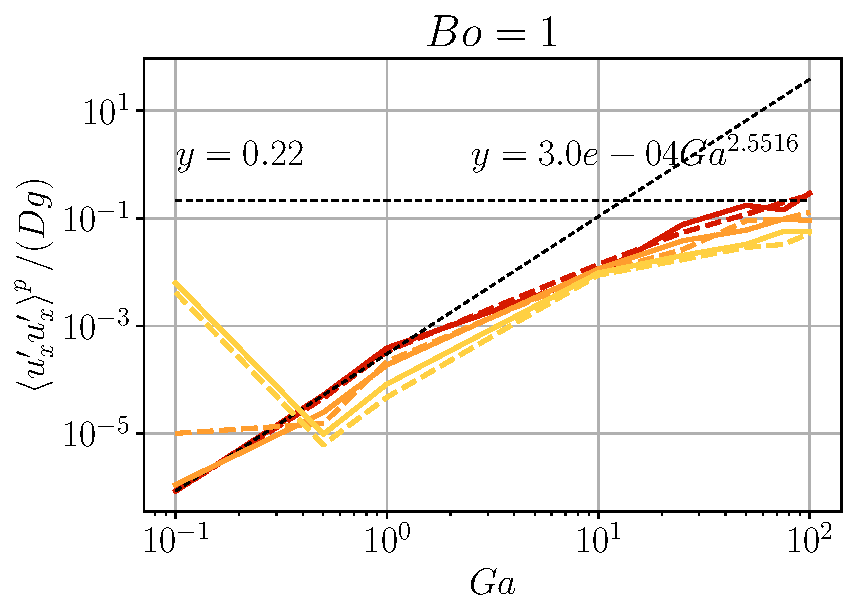
\includegraphics[height=0.20\textheight]{image/N_10/UU/UU_pxx_Bo_1.pdf}
    \caption{Fluid-phase average of the dimensionless velocity fluctuations. Dashed lines : $\mu_f = 0.42$, solid lines : $\mu_f = 0.042$, Dotted lines : asymptotic fit for $\phi = 0.05$ and $\mu_r = 0.42$. \textcolor{red}{\textbf{--}} : $\phi = 0.05$, \textcolor{orange}{\textbf{--}} : $\phi = 0.15$, \textcolor{yellow}{\textbf{--}} : $\phi = 0.25$} 
    \label{fig:UUp}
\end{figure} 
To estimate the value of the divergence of this tensor we consider a pipe flow where droplets are rising due to the gravity. 
Let's take a point far from a wall in our macroscopic medium. 
There, the Galileo number could be $Ga = 100$.
At the wall there are no velocity, thus, the pseudo turbulent tensor and the velocities are both null.   
Therefore, 
\begin{equation*}    
    \left(\bm{\nabla} \cdot \left<\bm{u}'\bm{u}'\right>^f \right)_j = \frac{<u_j' u_j'>^f}{\mathcal{L}}
\end{equation*}
In our case the scaling gives us a maximum of $10^{-2}$. 
If we compare this results to the drag force terms seen in the previous section we get an order of magnitude of two decades.
Therefore, this closure term has its importance, Nevertheless it might be negligible at this range of $Ga$. 
The last, fluctuation closure term that we can evaluate, is the one in \ref{eq:Iavg}, namely, 
\begin{equation}
    \bm{\nabla}\cdot(n\left<\bm{\omega'u'}\right>^p)_j 
    = \frac{\partial <\omega_i' u_j'>^f}{\partial x_i}.
\end{equation}
In 2D the derivative of the fluctuation will be inevitably null since $\bm{u}$ is function of $x$ and $y$, while $\bm{\omega}$ is defined on the $z$ axis.


\subsubsection{The coalescence kernel}
To close to coalesce kernel we need correlation on the collision frequency and time of contact. 
Nevertheless, in \ref{chap:avg} we that the present model were designed under different assumptions depending on the collision behavior of the pair of droplets.
Therefore, we are going to study the behavior of the pairwise interaction together with the collision frequency. 
This way we can define properly the nature of the average interaction and give the value of the frequency. 

\tb{\subsubsection{Radial density function}}
\begin{figure}[h!]
    \centering
    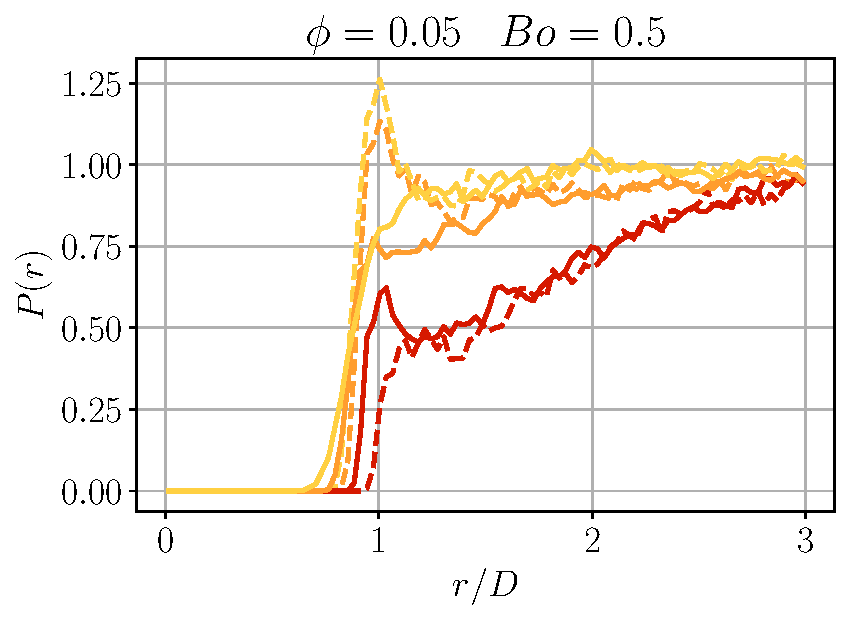
\includegraphics[height=0.15\textheight]{image/N_10/radial/probarBo0_5PHI0_05.pdf}
    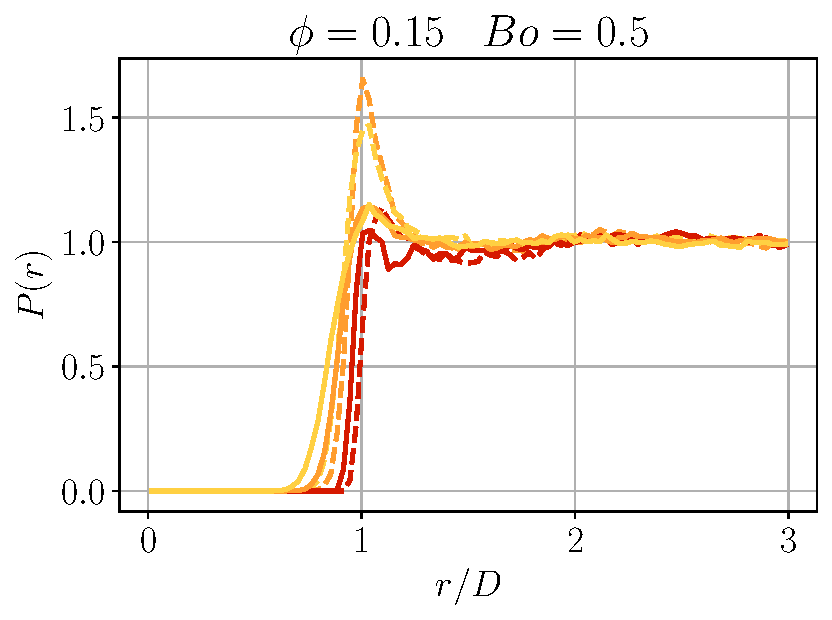
\includegraphics[height=0.15\textheight]{image/N_10/radial/probarBo0_5PHI0_15.pdf}
    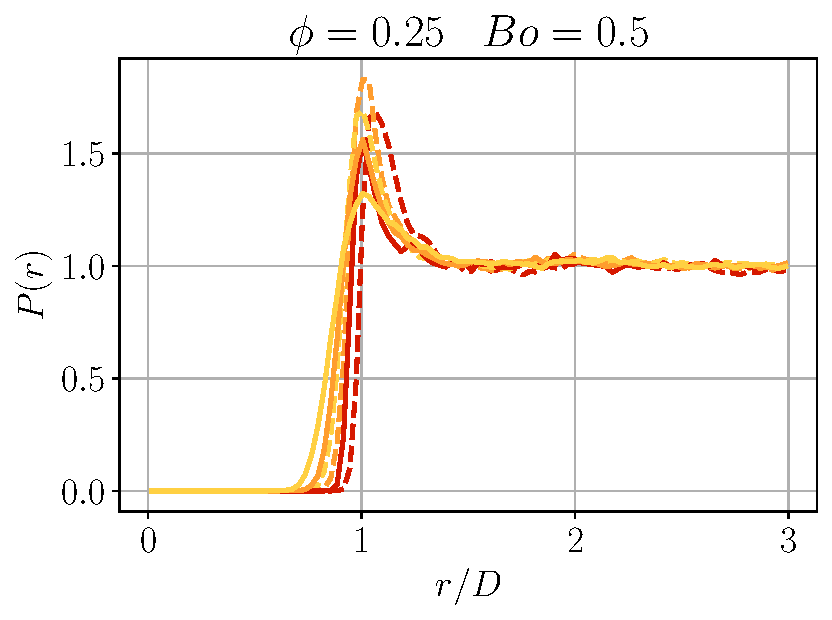
\includegraphics[height=0.15\textheight]{image/N_10/radial/probarBo0_5PHI0_25.pdf}
    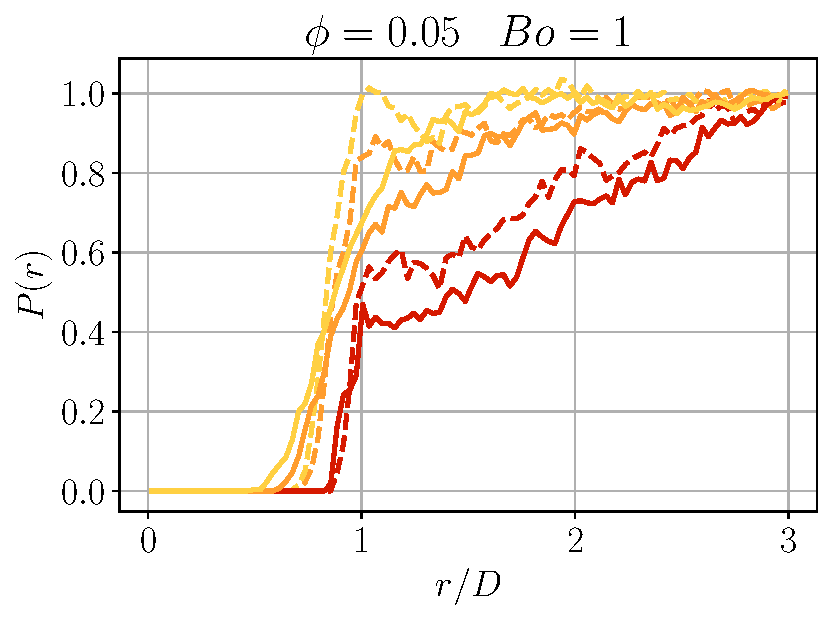
\includegraphics[height=0.15\textheight]{image/N_10/radial/probarBo1PHI0_05.pdf}
    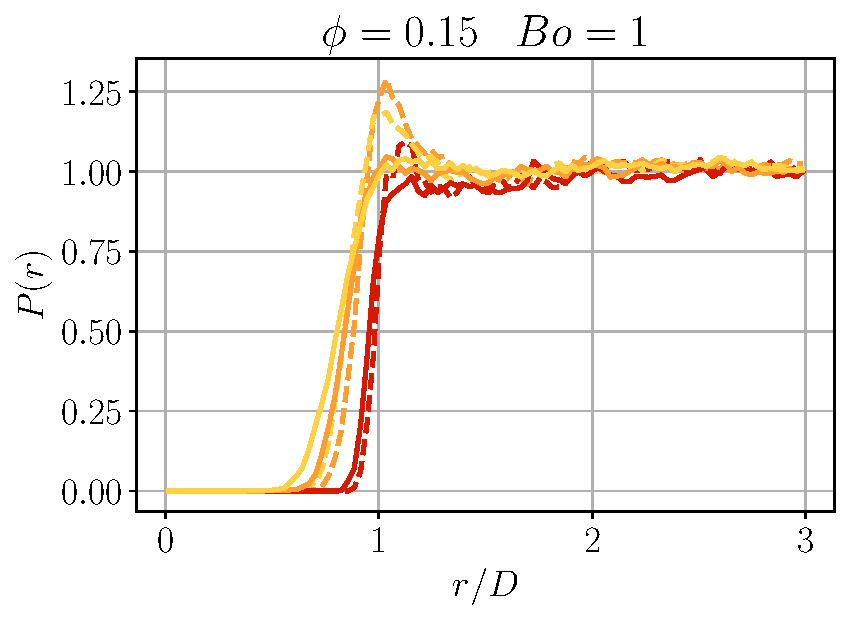
\includegraphics[height=0.15\textheight]{image/N_10/radial/probarBo1PHI0_15.pdf}
    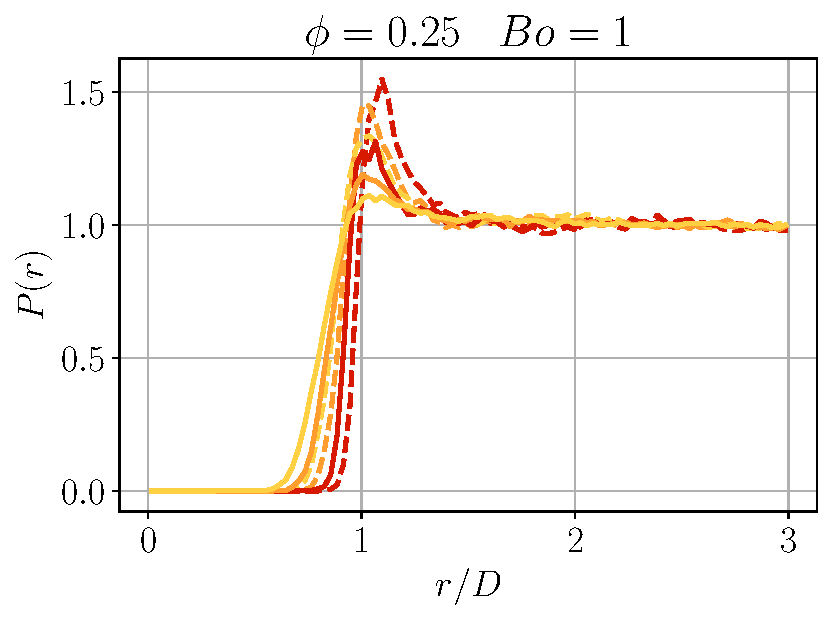
\includegraphics[height=0.15\textheight]{image/N_10/radial/probarBo1PHI0_25.pdf}
    \caption{Radial distribution function in terms of the nearest particle distance $d_{nbr}$. Dashed lines : $\mu_f = 0.042$, solid lines : $\mu_f = 0.42$.} 
    \label{fig:Pr}
\end{figure} 



\subsubsection{Pairwise interaction}
Let's $\Phi_\alpha$ being an internal property of a droplet, it could be the velocity $\bm{u}_\alpha$ or the deformation $\mathcal{G}_\alpha$ etc\ldots. 
Here, we are interested in the value of a given property $\Phi_\alpha$, knowing that the particle $\alpha$ is at a distance $d_{nbr}$ from its nearest neighbor, the particle $\beta$.
If we look for distances, $d_{nbr}$, small enough, we can determine the value of a parameter $\Phi_\alpha$ while the particle is in contact or close contact to another.
Similarly, we also can determine the average value of a property knowing the nearest neighbor is far from the particle $\alpha$. 
The value of the property $\Phi_\alpha$ knowing $d_{nbr}$ will be noted, $\Phi_\alpha(d_{nbr})$. 
The probability density function giving the number of event of a particle having a neighbor at a distance, $d_{nbr}$, considering all time and particles, is noted $P(d_{nbr})$.
Now, we apply ensemble average on the $\Phi_\alpha(d_{nbr})$ for each particle and all time.
Therefore, we define the function $\Phi(d_{nbr})$ as the average property of a particle knowing the distance with the nearest neighbor.

Lets being by looking at the probability density function $P(d_{nbr})$.
On \ref{fig:Pdmin} we can observe that similarly to the particle radial function the number of event tend to $0$ when $d_{nbr} \rightarrow 0$.
Also, the number of event goes to $0$ when $d_{nbr} \rightarrow \Delta P$
(we recall that $\Delta P$ is the averaged distance in the homogeneous configuration).
Therefore, for dilute suspension (i.e. $\phi =0.05$) the maximum $d_{nbr}$ is greater than for dense suspension. 
\begin{figure}[h!]
    \centering
    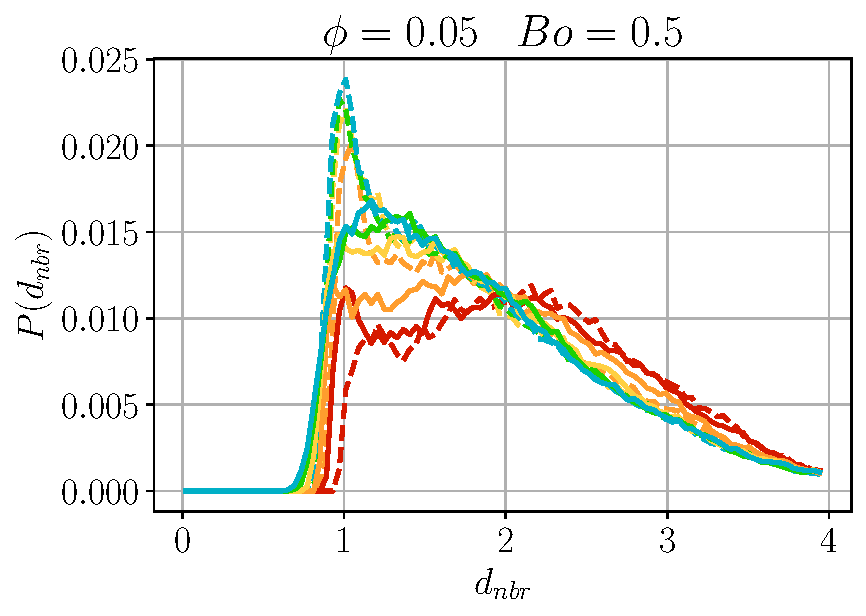
\includegraphics[height=0.15\textheight]{image/N_10/Pcond/probaNBo0_5PHI0_05.pdf}
    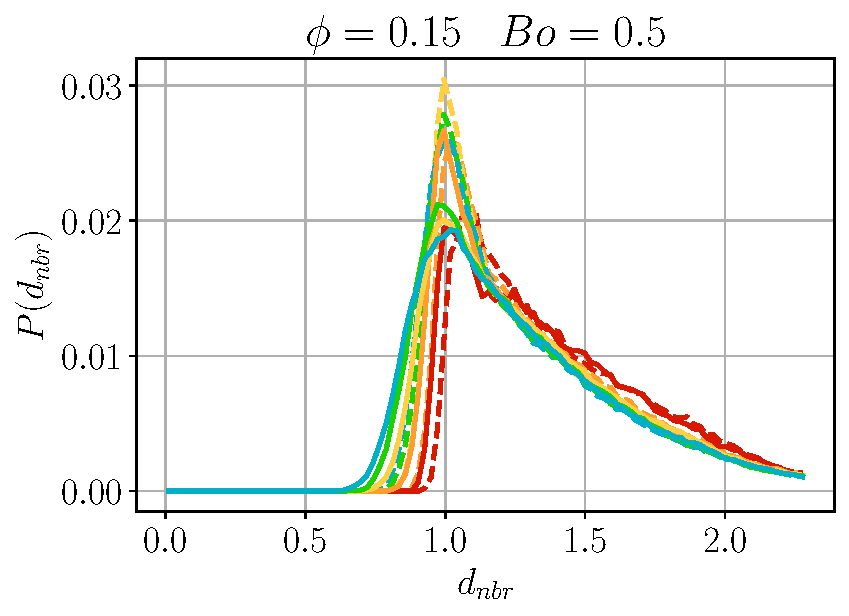
\includegraphics[height=0.15\textheight]{image/N_10/Pcond/probaNBo0_5PHI0_15.pdf}
    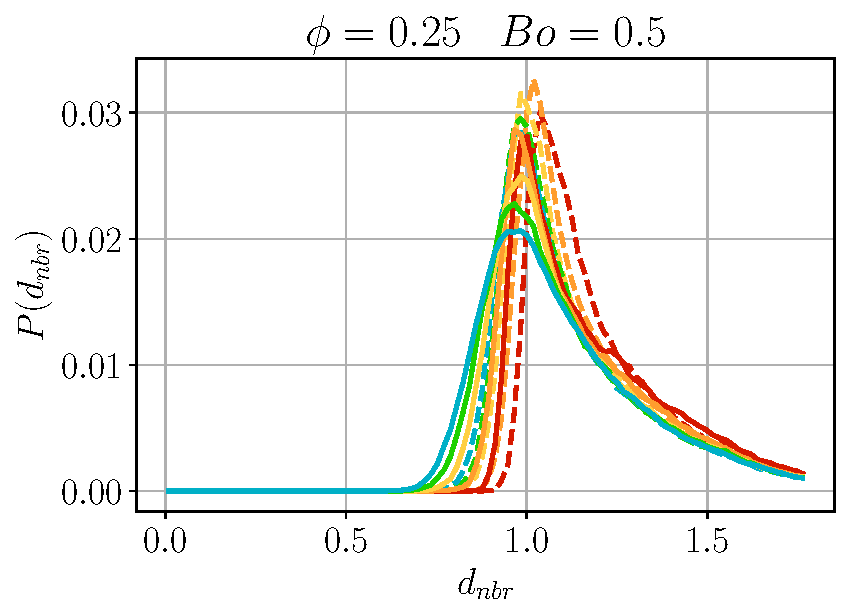
\includegraphics[height=0.15\textheight]{image/N_10/Pcond/probaNBo0_5PHI0_25.pdf}
    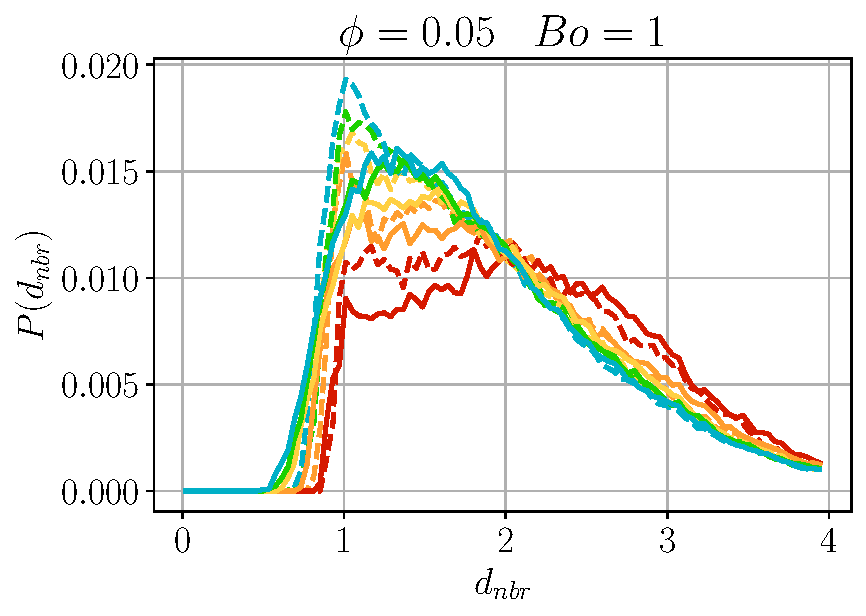
\includegraphics[height=0.15\textheight]{image/N_10/Pcond/probaNBo1PHI0_05.pdf}
    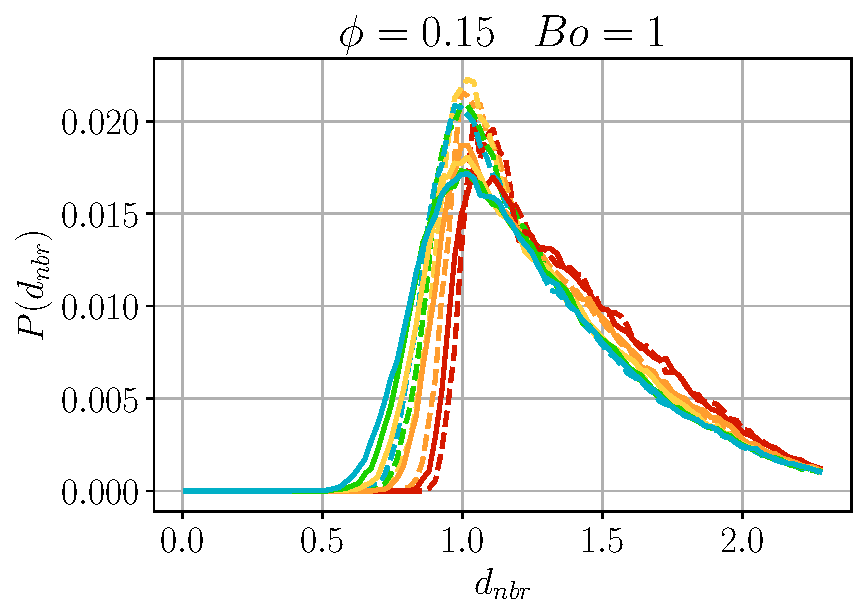
\includegraphics[height=0.15\textheight]{image/N_10/Pcond/probaNBo1PHI0_15.pdf}
    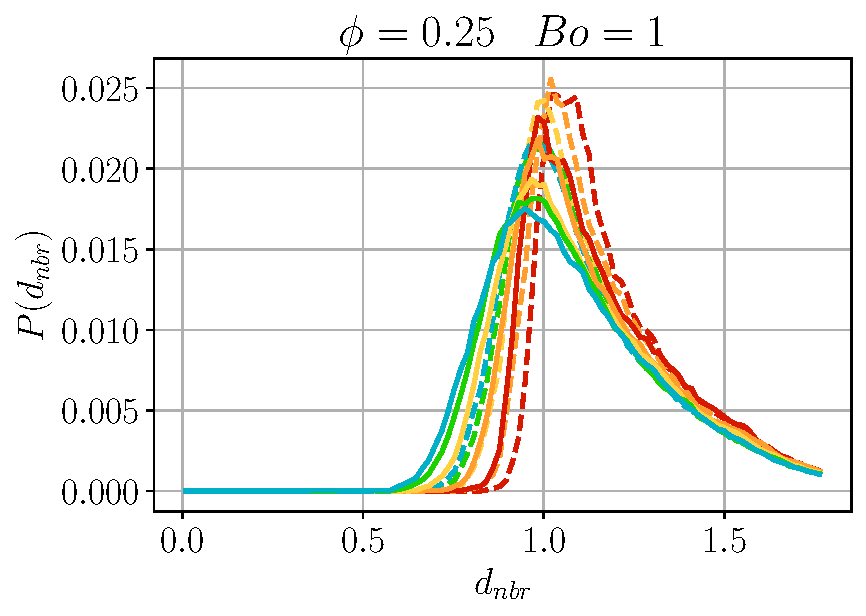
\includegraphics[height=0.15\textheight]{image/N_10/Pcond/probaNBo1PHI0_25.pdf}
    \caption{Probability density function in terms of the nearest particle distance $d_{nbr}$. Dashed lines : $\mu_f = 0.042$, solid lines : $\mu_f = 0.42$.} 
    \label{fig:Pdmin}
\end{figure} 
Before all else, it is obvious that the simulation with low \textit{Galileo number} have a maximum for considerably greater $d_{nbr}$. 
This fact testifies that the collision frequency is way lower than for the greater $Ga$. 
Besides, it also means that the set isn't representative to study the close particle interaction since the number of event is too low when $d_{nbr}\approx D$. 
Therefore, in the following we won't consider the low \textit{Galileo number} cases when looking at close interactions.
Regarding high \textit{Galileo number} we can see that the higher $Ga$ is the smaller $Ga$ is. 
Indeed, we can see that for the greatest $Ga$, $d_{nbr}/D$ reaches $0.8$.
The droplet fraction $\phi$ modify significantly the shape o the distribution function. 
Indeed, on can note that for low $\phi$ the distribution flatten, while for higher $\phi$ it is sharper. 
Besides, the number of event is significantly more abundant for high $\phi$.
Again, the change in $Bo$ number and $\mu_r$ seems to have a limited impact on the distribution. 
Ultimately no significant parameter seems to influence the shape of the probability density function apart from $Ga$ and $\phi$. 

Next, we evaluate the cinematic quantity, i.e. the averaged velocity $\bm{u}(d_{nbr})$. 
We recall that we will be looking only at the $Ga \in [10;100]$ since the lower $Ga$ are not representative. 
But before note that some quantities are proper to the particle, as the deformation for example, while others quantities need to be evaluated relatively to the nearest neighboring particle. 
It is the case for the velocity of the center of mass $\bm{u}_\alpha$.
Indeed, if we want to evaluate properly the cinematic between two particles we need to correlate the relative velocities of the particles to $d_{nbr}$. 
Therefore, on \ref{fig:Pvrel}(a), (b) and (c) we can observe the relative velocity between two particles knowing the distance between one and the nearest neighbor. 
    \begin{figure}[h!]
        \centering
        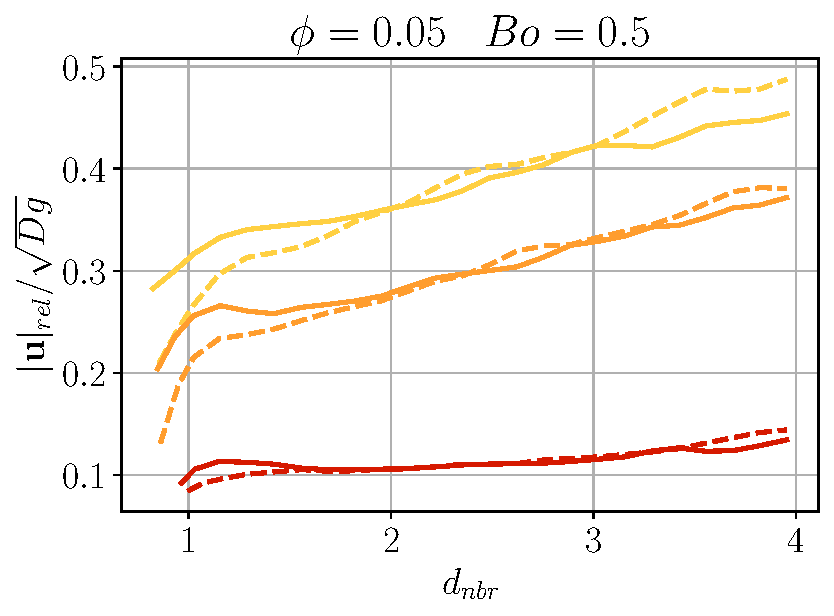
\includegraphics[height=0.16\textheight]{image/N_10/Pcond/probav_relBo0_5PHI0_05.pdf}
        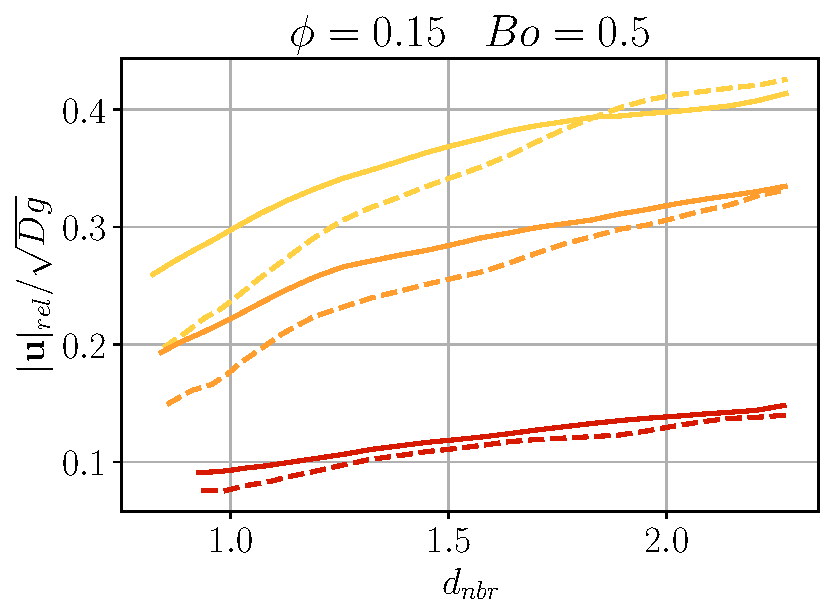
\includegraphics[height=0.16\textheight]{image/N_10/Pcond/probav_relBo0_5PHI0_15.pdf}
        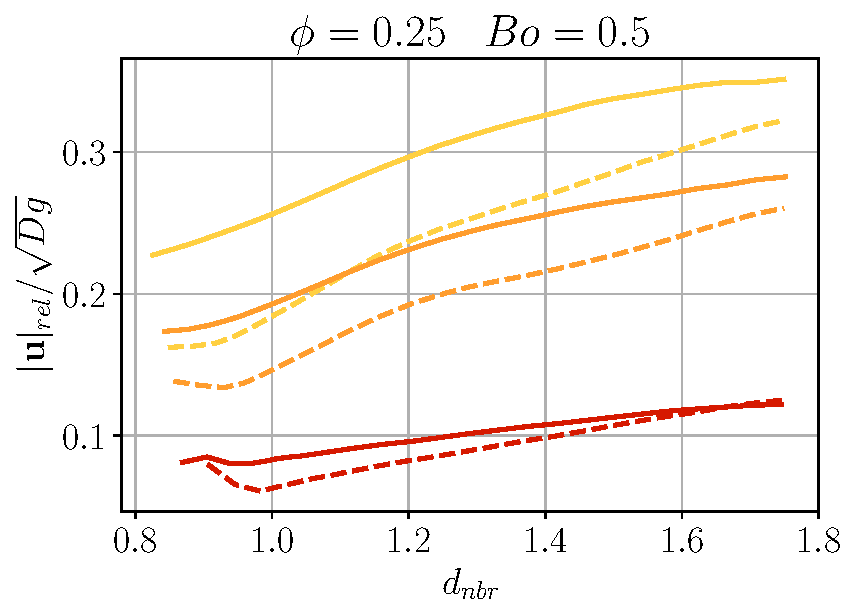
\includegraphics[height=0.16\textheight]{image/N_10/Pcond/probav_relBo0_5PHI0_25.pdf}

        \hspace{3cm}(a)\hfill(b)\hfill(c)\hspace{3cm}
        
        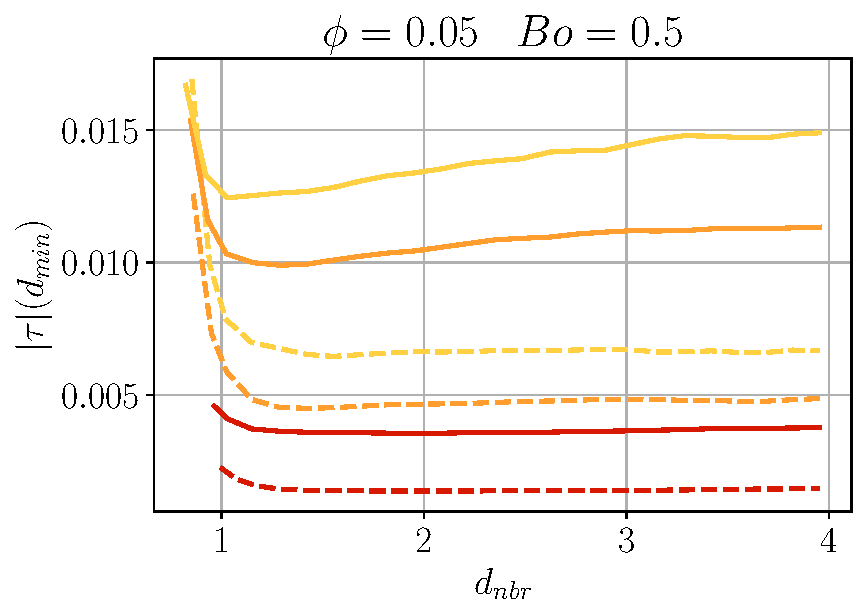
\includegraphics[height=0.16\textheight]{image/N_10/Pcond/probadissBo0_5PHI0_05.pdf}
        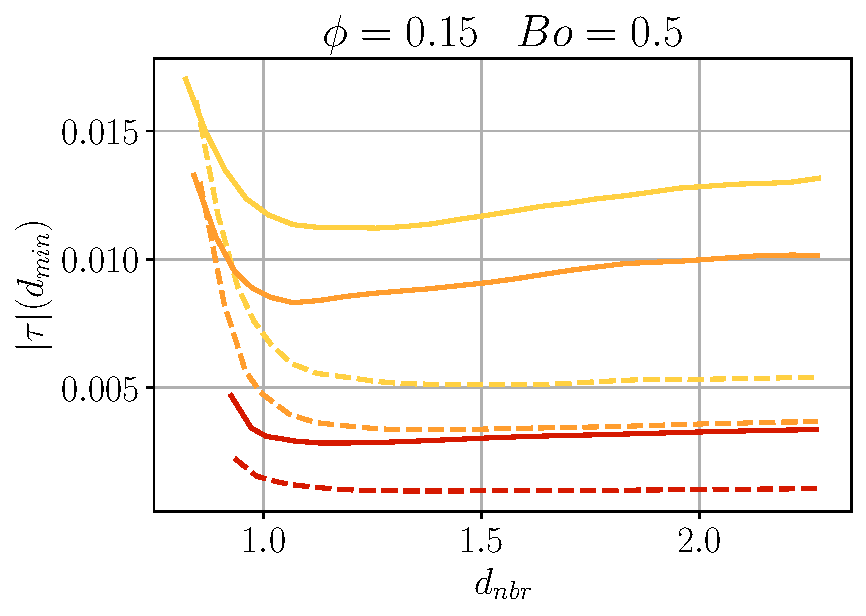
\includegraphics[height=0.16\textheight]{image/N_10/Pcond/probadissBo0_5PHI0_15.pdf}
        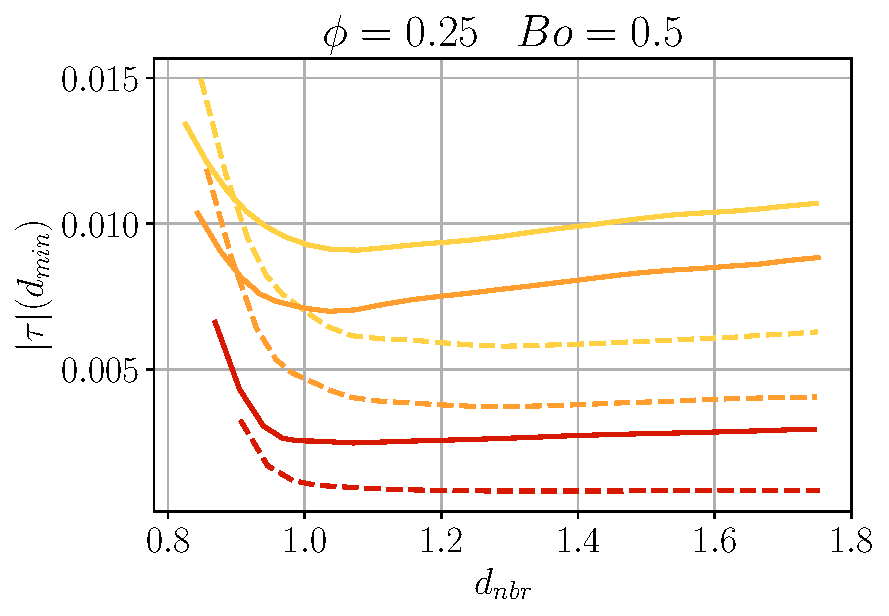
\includegraphics[height=0.16\textheight]{image/N_10/Pcond/probadissBo0_5PHI0_25.pdf}
        
        \hspace{3cm}(d)\hfill(e)\hfill(f)\hspace{2.5cm}
        
        \caption{(top) Relative velocity (bottom) dissipation in terms of the nearest particle distance $d_{nbr}$. Dashed lines : $\mu_f = 0.042$, solid lines : $\mu_f = 0.42$.} 
        \label{fig:Pvrel}
    \end{figure} 
This figure shows clearly that the closer the particles get the smaller the norm of the relative velocity is which is trivial.
We can also note on \ref{fig:Pvrel}(d), (e) and (f) that the norm of the dissipation, namely, $2\tau = \nabla u + (\nabla u)^T$ increase at the contact. 
Indeed, flow low values of $d_{min}$ the dissipation increase due to the contact and deformation of the particles.   
Even through \ref{fig:Pvrel} provide a good scaling for the interaction velocity, it doesn't describe the arrangement of the two drops during a collision. 
Indeed, the theoretical models seen \ref{chap:avg} considered either a constant velocity, or a constant forces during the interaction of two particles.
The latter model can be discarded considering the preceding observation.
Besides, those models considered cases with tangential or  normal relative velocity. 
Therefore, it is of interest to study the orientation of those interactions while considering the value of the velocities during the approach.

We consider the following geometrical parameters (see \ref{fig:para}) to study the averaged relative potions and motions of the pairs of droplets. 
\begin{figure}[h!]
    \centering
    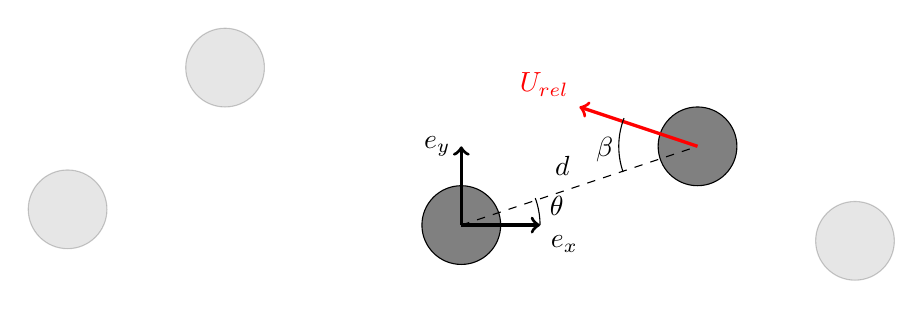
\begin{tikzpicture}
        \draw[fill=gray](0,0)circle (0.5);
        \draw[fill=gray](3,1)circle (0.5);
        \draw[fill=gray,opacity=0.2](5,-0.2)circle (0.5);
        \draw[fill=gray,opacity=0.2](-3,2)circle (0.5);
        \draw[fill=gray,opacity=0.2](-5,0.2)circle (0.5);
        \draw[dashed](0,0)--(3,1)node[midway,above left]{$\bm{d}$};
        \draw[very thick,->,red](3,1)--++(-1.5,0.5)node[above left]{$\bm{U_{rel}}$};
        \draw[very thick,->](0,0)--++(1,0)node[below right]{$\bm{e_x}$};
        \draw[very thick,->](0,0)--++(0,1)node[left]{$\bm{e_y}$};
        \draw(3,1)++(199:1)node[above left]{$\beta$} arc(199:159:1);
        \draw(0,0)++(0:1)node[above right]{$\theta$} arc(0:20:1);
    \end{tikzpicture} 
    \caption{Scheme of a drop labeled $\alpha =1$ and its nearest neighbor $\alpha = 2$. The velocity is considered in the frame of the first drop thus, $\bm{u}_rel =  \bm{u}_2-\bm{u}_1$ with $\bm{u}_1$ and $\bm{u}_2$ being respectively the velocities of the first and second drop. The distance between the two drop, $\bm{d} = \bm{y}_2 -\bm{y}_1$, and its norm $d_{nbr} = |\bm{d}|$. }
    \label{fig:para}
\end{figure}
Any of the parameters \ref{fig:scheme} can be associated to the particle at the origin. 
Thus, for any particle $\alpha$ at any time $t$ we can define a $\beta_{\alpha}$, $\theta_{\alpha}$ and so on. 
All those parameters can be gathered together in inside a unique vector, namely $\bm{\lambda} = (\theta,\beta,d_{nbr},u_{rel})$ 
Then, the probability density function, $P(\bm{\lambda})$, is defined such that, $P(\bm{\lambda})d\lambda$, is the probability of finding a pair of particles being in the configuration $\lambda$.  
Hence, it is possible to define subgroups of this function by integrating it over a set of parameters. 
For example, if we are interested in the angle dependency only, we can define the sub-distribution,
\begin{equation}
    P_{\beta\theta}(\beta,\theta) = \iint P(\bm{\lambda}) du_{rel} dd_{ndr}.
\end{equation}
Similarly, we could define any other density distribution function by integrating over the other variables.
So $P_{\bm{p}}(\bm{p})$ is the probability density function of the set of variable $\bm{p}$.
On the above example $\bm{p} = (\theta,\beta)$. 
So, we start by investigating the distribution $P_{\beta\theta}(\beta,\theta)$. 
The angle $\beta$ represent the angle of approach since it is taken between the vector $\bm{d}$ and the relative velocity $\bm{u}_{rel}$. 
Hence, when $\beta = \pi/2$ the approach is tangential, and when $\beta= 0$ or $\pi$ it is a normal approach.  
Also, the angle $\theta$ will be useful to investigate the direction of the collision. 
Indeed, for poly-disperse flow we could remark that the bigger drops had a tendency to hit the smaller from the bot due to the difference in rising velocity.
Here, we treat only mono disperse cases, still it is of interest to check if a trend emerges. 
% \begin{figure}[h!]
%     \centering
%     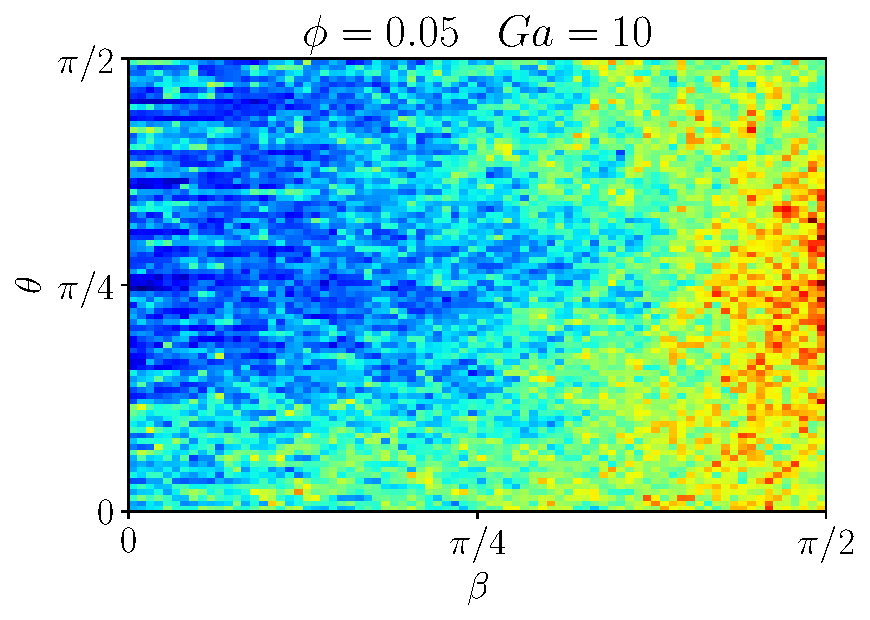
\includegraphics[height = \size]{image/N_10/beta/2DMAP_beta_theta_dmin_10_Bo0_5PHI0_05mu_r0_042Ga10.pdf}
%     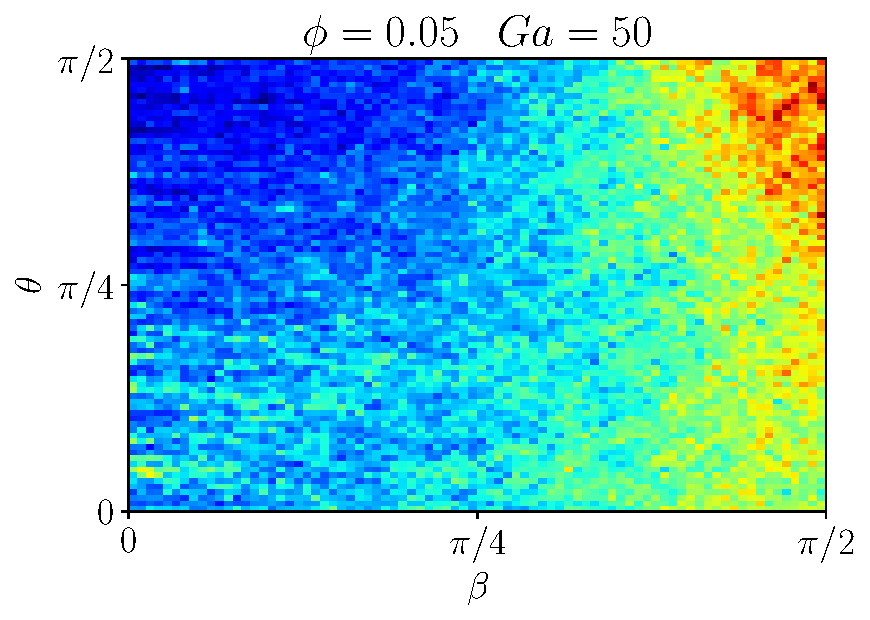
\includegraphics[height = \size]{image/N_10/beta/2DMAP_beta_theta_dmin_10_Bo0_5PHI0_05mu_r0_042Ga50.pdf}
%     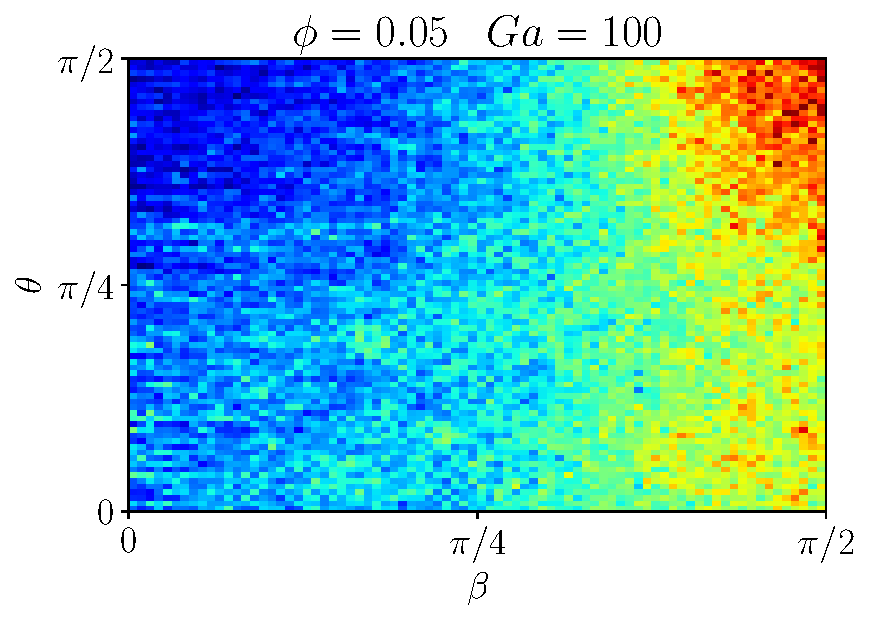
\includegraphics[height = \size]{image/N_10/beta/2DMAP_beta_theta_dmin_10_Bo0_5PHI0_05mu_r0_042Ga100.pdf}
%     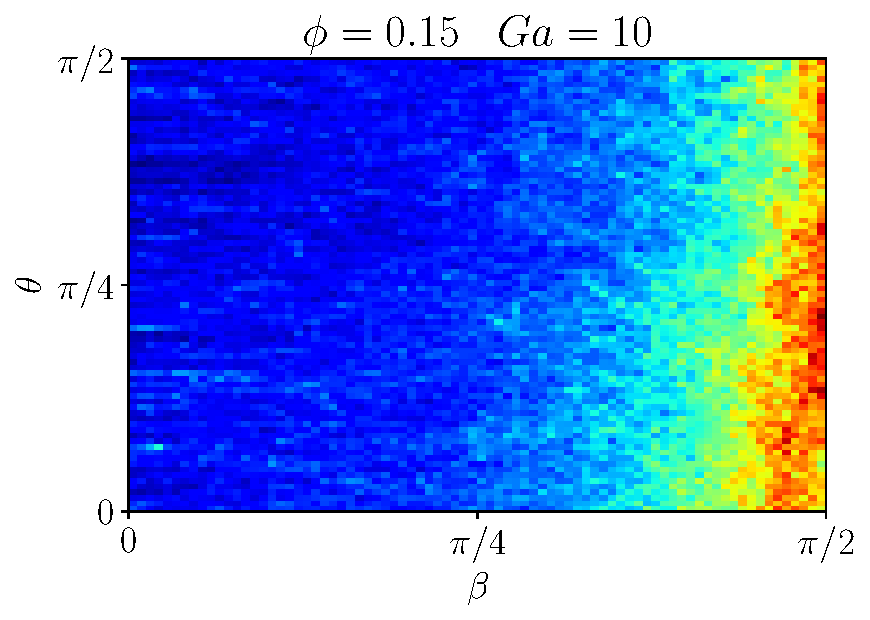
\includegraphics[height = \size]{image/N_10/beta/2DMAP_beta_theta_dmin_10_Bo0_5PHI0_15mu_r0_042Ga10.pdf}
%     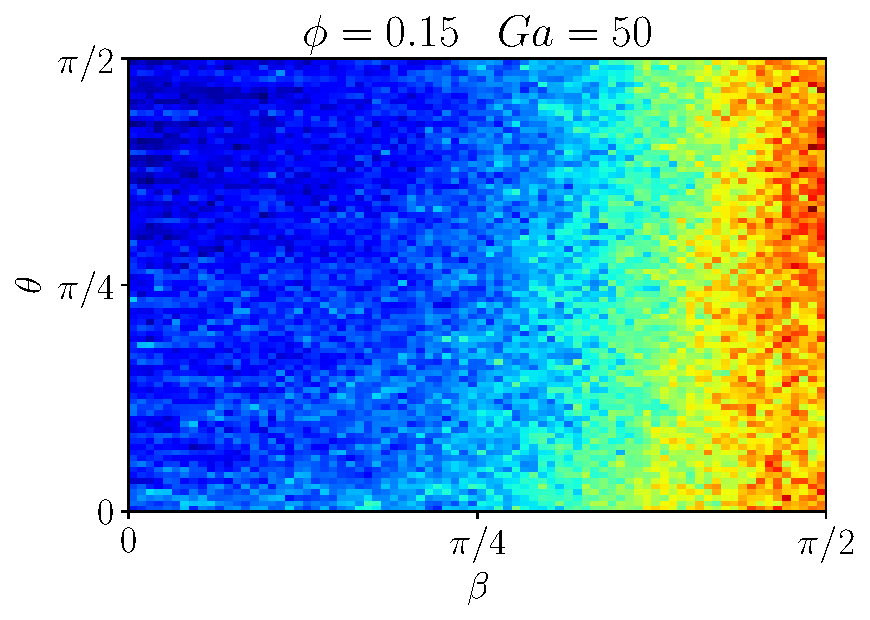
\includegraphics[height = \size]{image/N_10/beta/2DMAP_beta_theta_dmin_10_Bo0_5PHI0_15mu_r0_042Ga50.pdf}
%     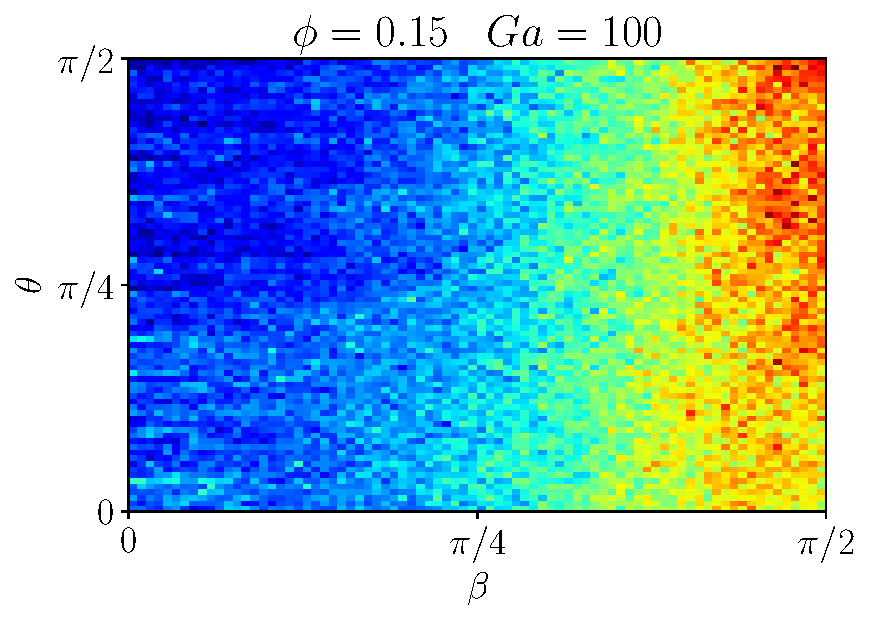
\includegraphics[height = \size]{image/N_10/beta/2DMAP_beta_theta_dmin_10_Bo0_5PHI0_15mu_r0_042Ga100.pdf}
%     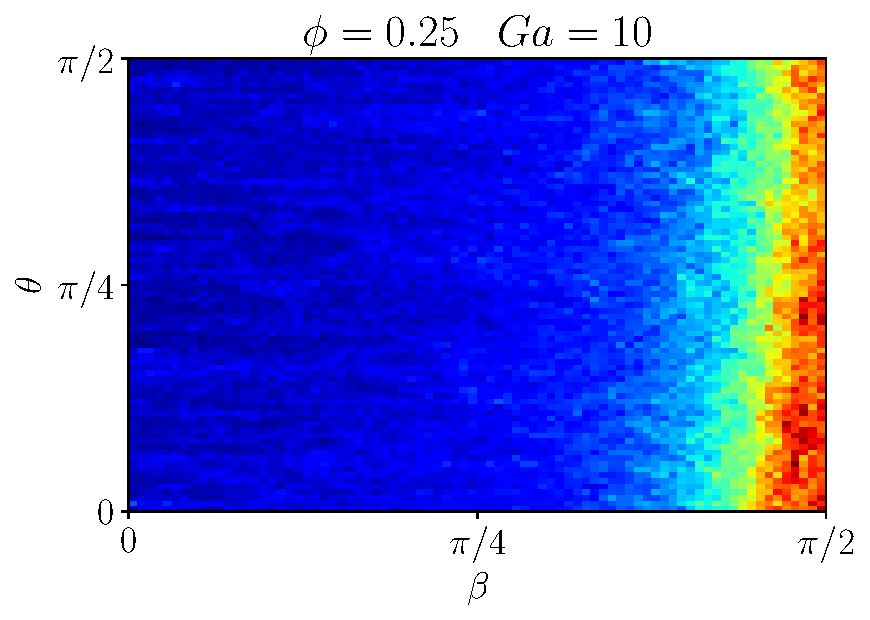
\includegraphics[height = \size]{image/N_10/beta/2DMAP_beta_theta_dmin_10_Bo0_5PHI0_25mu_r0_042Ga10.pdf}
%     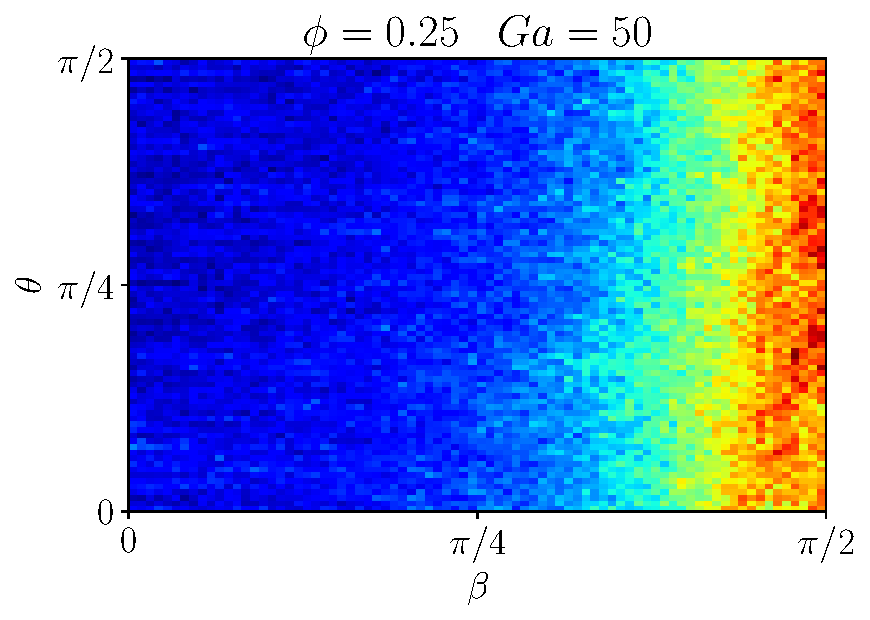
\includegraphics[height = \size]{image/N_10/beta/2DMAP_beta_theta_dmin_10_Bo0_5PHI0_25mu_r0_042Ga50.pdf}
%     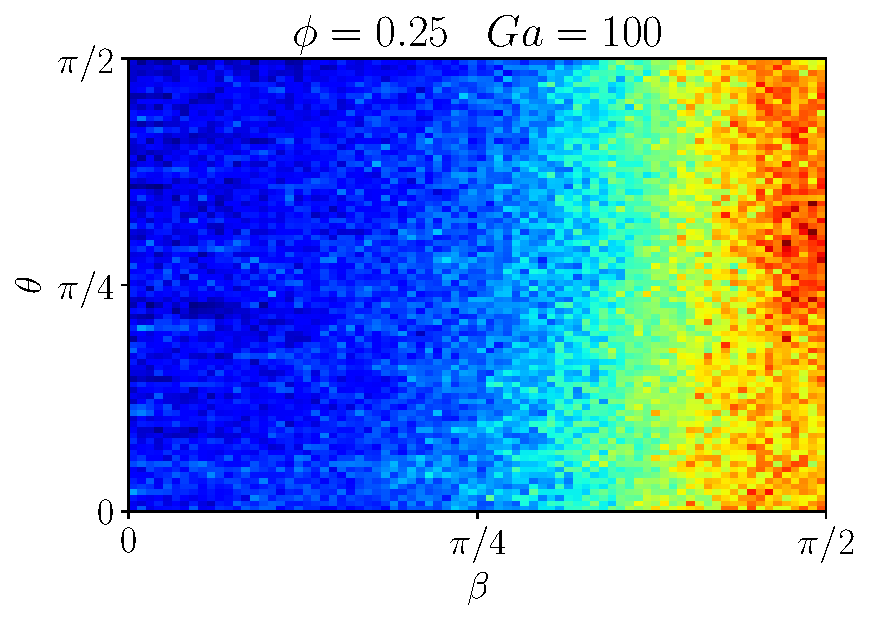
\includegraphics[height = \size]{image/N_10/beta/2DMAP_beta_theta_dmin_10_Bo0_5PHI0_25mu_r0_042Ga100.pdf}
%     \caption{2 plots of $P_{\beta\theta}(\beta,\theta)$ for different $\phi$ and $Ga$ at $Bo = 0.5$ and $\mu_r = 0.042$. The color represents the density, it goes from blue meaning $P_{\beta\theta}(\beta,\theta)= P_{min}$, to red meaning $P_{\beta\theta}(\beta,\theta) = P_{max}$. The different plots are label from left to right and from top to bottom with the letters (a) to (i).} 
%     \label{fig:beta_theta_2D}
% \end{figure} 
On \ref{fig:beta_theta_2D} we can observe the density distribution $P_{\beta\theta}$ for different $\phi$ and $Ga$. 
We can clearly identify two trends. 
The first one is depicted at high drop volume fraction and  high $Ga$, \ref{fig:beta_theta_2D}(i).
It shows that the distribution is clearly independent of the angle $\theta$.
In other words, the distribution, $P_{\beta}$ evaluated at $\theta_i$, or $P_{\beta}(\theta=\theta_i)$ is constant of all $\theta_i$. 
Moreover, the distribution of $\theta$ and $\beta$ independently of one another, is respectively uniform and Gaussian shaped around $\beta = \pi/2$ (see \ref{ap:dist} \ref{sec:dist_theta}).
Besides, it can be seen that the standard deviation  about $\beta$ is clearly increasing with $Ga$. 
So, we can conclude that for high $\phi$ the direction of the contact (i.e. $\theta$) is rather random and the nature of the interaction is tangential (since $\beta \approx \pi/2$). 
For low volume fraction of drops and rather high $Ga$ (plots (b) and (c) \ref{fig:beta_theta_2D}) we can distinguish a pic of density at $\theta = \pi/2$ and $\beta = \pi/2$. 
While, in \ref{ap:dist} \ref{sec:dist_theta}, we show that the distribution of $P_\theta$ is still uniform. 
Therefore, we can conclude that $\beta$ is centered around $\pi/2$ at $\theta \approx \pi/2$ and uniform when $\theta = 0$ or $\pi$. 
In others words, the interactions are rather tangential for vertical contacts and random when the approach is horizontal. 
Finally, for the plot (a) the distribution seem random and nearly uniform for both variables. 
All the others values of $Bo$ and $mu_r$ are shown in the figures in \ref{ap:dist} section \ref{sec:dist_beta_theta}.
Even though  those parameters influence lightly the distribution, one can note that the global trend is still preserved.

Next we study the dependency of the angle $\beta$ with the norm of the distance to the closest neighbor, i.e. $d_{nbr}$.
Hence, we evaluate the probability density function $P_{\beta d_{nbr}}(\beta, d_{nbr})$ according to the definition mentioned earlier. 
% \begin{figure}[h!]
%     \centering
%     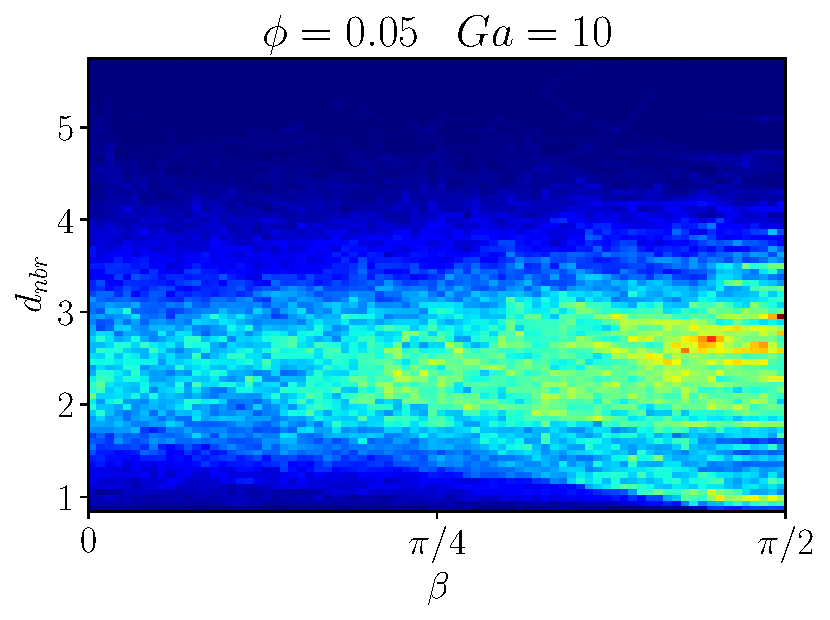
\includegraphics[height = \size]{image/N_10/beta/2DMAP_beta_distmin_dmin_10_Bo1PHI0_05mu_r0_42Ga10.pdf}
%     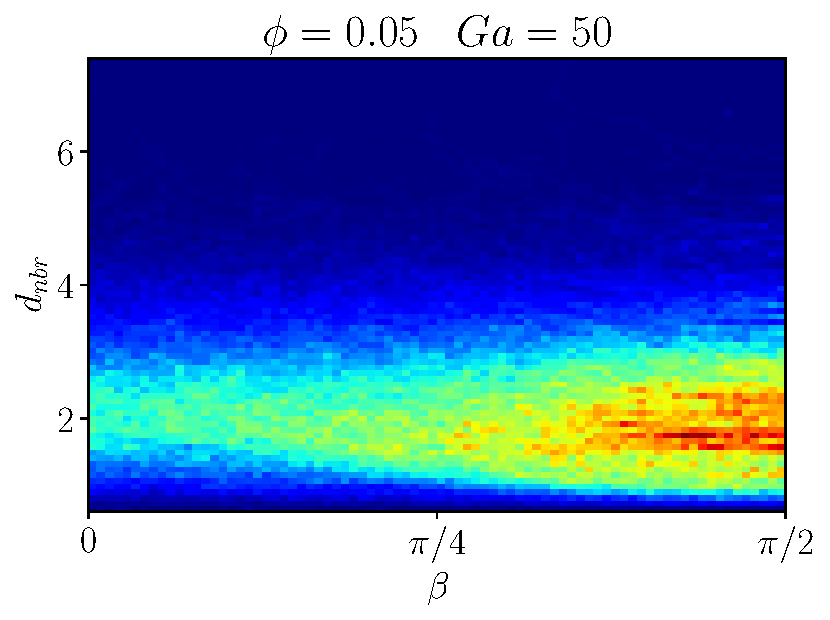
\includegraphics[height = \size]{image/N_10/beta/2DMAP_beta_distmin_dmin_10_Bo1PHI0_05mu_r0_42Ga50.pdf}
%     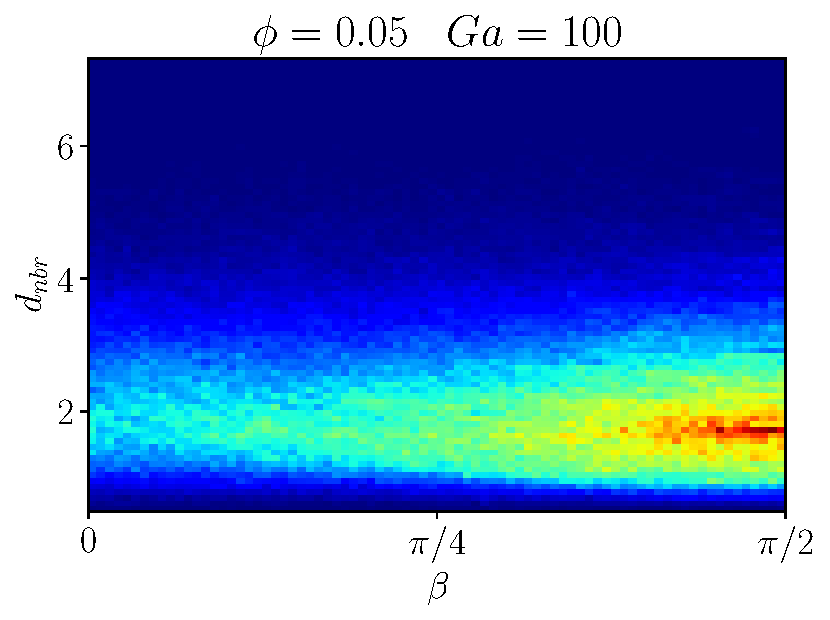
\includegraphics[height = \size]{image/N_10/beta/2DMAP_beta_distmin_dmin_10_Bo1PHI0_05mu_r0_42Ga100.pdf}
%     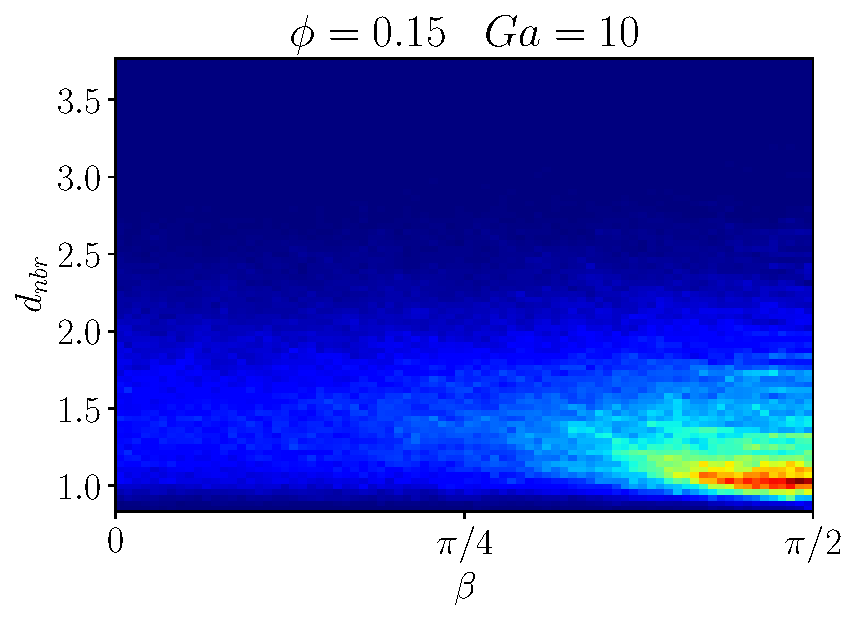
\includegraphics[height = \size]{image/N_10/beta/2DMAP_beta_distmin_dmin_10_Bo1PHI0_15mu_r0_42Ga10.pdf}
%     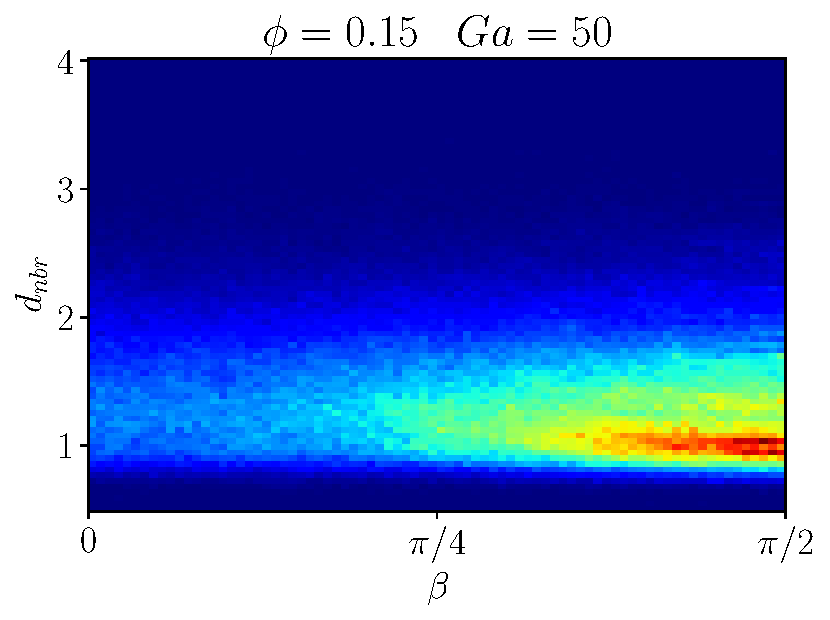
\includegraphics[height = \size]{image/N_10/beta/2DMAP_beta_distmin_dmin_10_Bo1PHI0_15mu_r0_42Ga50.pdf}
%     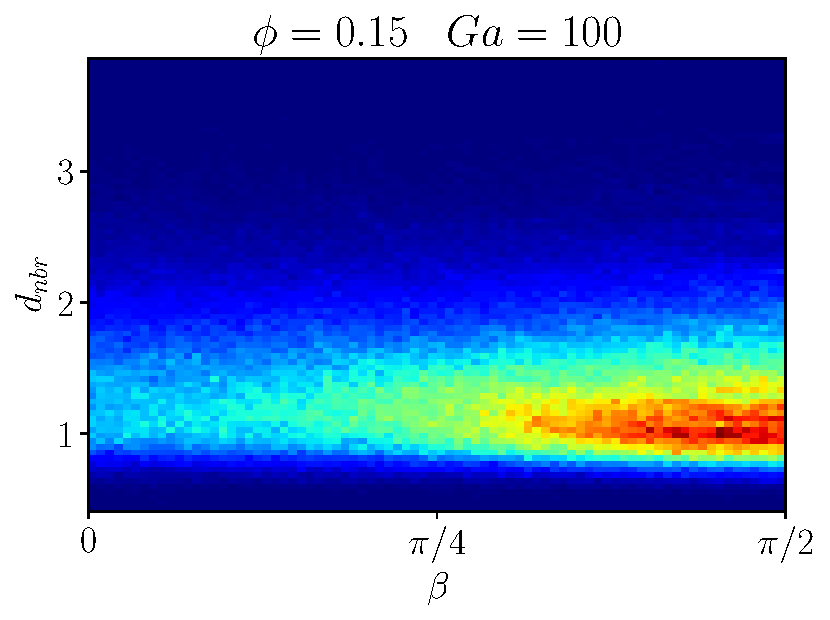
\includegraphics[height = \size]{image/N_10/beta/2DMAP_beta_distmin_dmin_10_Bo1PHI0_15mu_r0_42Ga100.pdf}
%     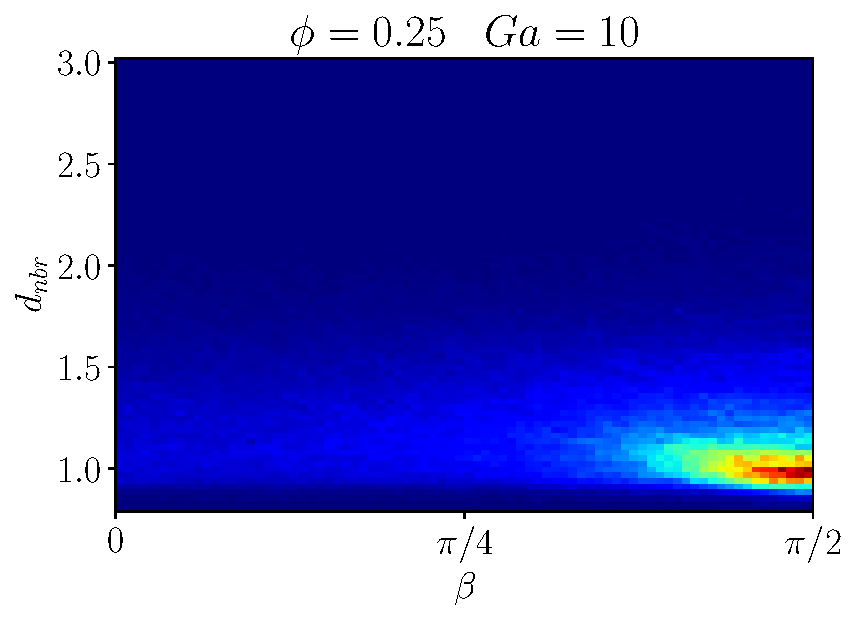
\includegraphics[height = \size]{image/N_10/beta/2DMAP_beta_distmin_dmin_10_Bo1PHI0_25mu_r0_42Ga10.pdf}
%     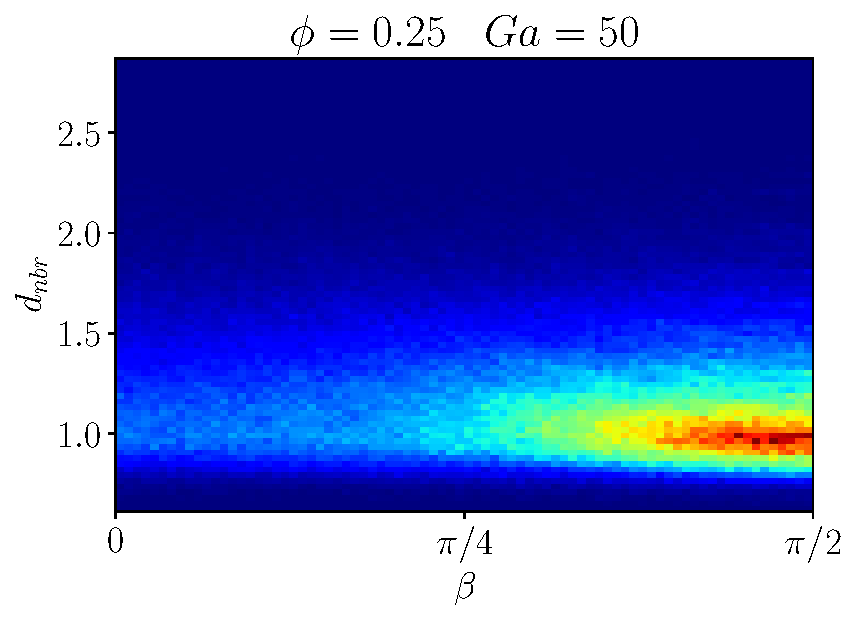
\includegraphics[height = \size]{image/N_10/beta/2DMAP_beta_distmin_dmin_10_Bo1PHI0_25mu_r0_42Ga50.pdf}
%     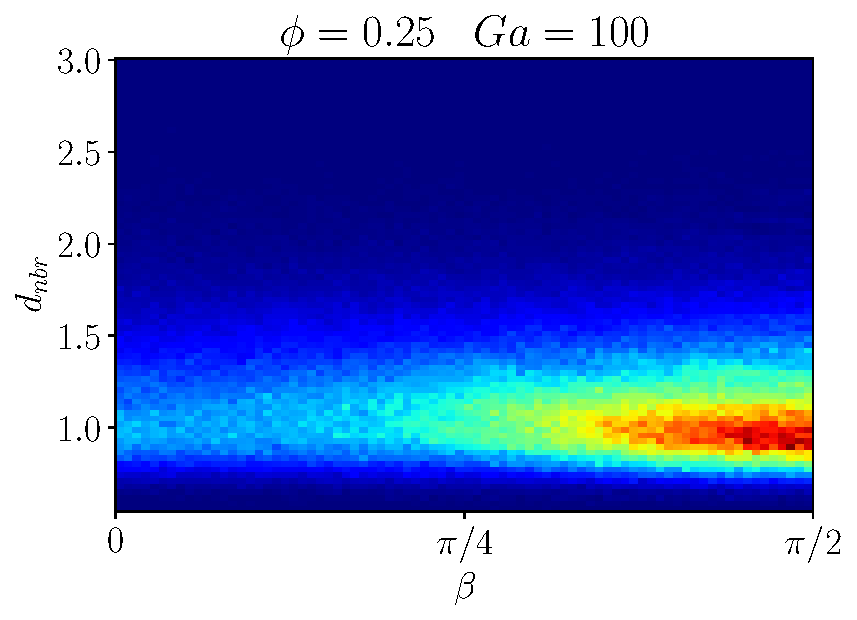
\includegraphics[height = \size]{image/N_10/beta/2DMAP_beta_distmin_dmin_10_Bo1PHI0_25mu_r0_42Ga100.pdf}
%     \caption{2 plots of $P_{\beta d_{nbr}}(\beta,d_{nrb})$ for different $\phi$ and $Ga$ at $Bo = 0.5$ and $\mu_r = 0.042$. The color represents the density, it goes from blue meaning $P_{\beta d_{nrb}}(\beta,d_{nrb})= P_{min}$, to red meaning $P_{\beta d_{nrb}}(\beta,d_{nrb}) = P_{max}$. The different plots are label from left to right and from top to bottom with the letters (a) to (i).} 
%     \label{fig:beta_distmin_2D}
% \end{figure} 
\ref{fig:beta_distmin_2D} shows clearly the dependency between the variables. 
Let's consider the \ref{fig:beta_distmin_2D}(d) for instance. 
If we look at the distribution $P_{\beta d_{nbr}}$ for rather low $d_{min}$, let's say $d_{min}\approx 2$.
Then, we can note that $P_{\beta d_{nbr}}(\beta, d_{nbr} = 2)$ is rather uniform since it has the same color all along the horizontal line $d_{min} = 2$.
On the contrary, the distribution  $P_{\beta d_{nbr}}(\beta, d_{nbr} = 1)$ is highly concentrated at $\beta \approx \pi/2$.
Hence, we can affirm that in average, the closer a particle get to another, the more probable it is that the relative motion becomes tangential.
In the previous paragraph we deduced that the motion were rather tangential relatively to the nearest neighbor, for any distance $d_{nbr}$.
Here, we confirm this tendency, and affirm that the standard deviation around $\beta =\pi/2$ shrink with decreasing $d_{nbr}$.
Depending on $\phi$ and $Ga$ one can note that the distribution more or less flattened.   
For $\phi = 0.05$ the distribution is spread out. 
This can be explained through the fact that in dilute suspensions it is more probable to find the nearest neighbor far from a given particle. 
Therefore, the behavior is rather random, hence the distribution is homogeneous or spread out. 
Nevertheless, we still observe the shrinking of $P_\beta$ for decreasing value of $d_{nbr}$ (it is particularly obvious on \ref{fig:beta_distmin_2D} (a)). 
For higher $\phi$ the whole distribution shrink in both direction, i.e. for $\beta$ and $d_{nbr}$.
Obviously, when $\phi$ increase, the $P_{d_{nbr}}$ shrink around $1$ since the particles are constantly closer to their neighbor (see  \ref{fig:Pdmin}). 
Then, as we already mention at small $d_{nbr}$ the distribution in $\beta$ shrink around $\pi/2$.
Consequently, for small $\phi$ the distribution shrink in both direction, i.e. the particles are often in contact and their relative motion is tangential. 
Lastly, we note that $P_{\beta d_{min}}$ spread out with respect to the variable $\beta$ for increasing $Ga$. 

Next, it is interesting to say a few words on the distribution, ($u_{rel}$,$\beta$) plotted \ref{fig:beta_u_rel_2D}. 
The norm of the relative velocity is in average higher for tangential interactions.
Moreover, we recall that tangential interaction are more likely to happen, therefore the normal interaction are less abundant and in average lower than for tangential interaction. 
Let's summarize all the comments made up to now. 
We have shown that the interaction orientation i.e. $\theta$ is random for the whole range of parameters.
Then, we prove that the interactions are in average tangential, except when the orientation is horizontal and the droplet fraction low, in which cases $P_\beta$ is nearly uniform. 
Regarding the dependency with the distance with the closest neighbor, we conclude that the smaller $d_{min}$ is the smaller the standard deviation of $P_\beta$ will be. 
Physically, it means that the majority of the closest interaction happen tangentially. 
Then we mentioned the fact that we reached higher velocities for tangential interaction than normal interactions. 
In the general case we could note that the dispersion of $P_\beta$ increase with increasing $Ga$, $Bo$ and $\mu_r$ (see \ref{fig:beta_bomu}). 
Which is easily explainable, for high $Ga$ the momentum is higher and the drops interactions more \textit{straight}. 
For $Bo$ the increasing deformability of the drops could allow more close normal contacts.
For $\mu_f$ it is less obvious, we cannot conclude \textcolor{blue}{yet}. 


\subsubsection{Time and frequency of the contacts}
Now that we have a general idea of the classic contact architecture it is of interest to study the time of interaction. 
Indeed, as presented in \ref{chap:avg} the probability of coalescence highly depend on the time of interaction of the droplets. 
Nevertheless, it is not trivial to define the meaning of the nature of a contact, i.e. when do we consider that the droplets are in close contact ?
\tb{This question will be answered latter}, but for now we consider that a contact begin when the two droplets are at a distance less than one diameter. 
On \ref{fig:time_of_c} we can observe the mean value of the time of contact for each case.
It turns out that they all have the same tendency relatively to the \textit{Galileo} number. 
\tb{We can observe that the normalization with the inertial time gives a dependency with $Ga$ which is inversely proportional.}
\tb{For low $Ga$ if we norm by the viscous time we get another tendency.}
\begin{figure}[h!]
    \centering
    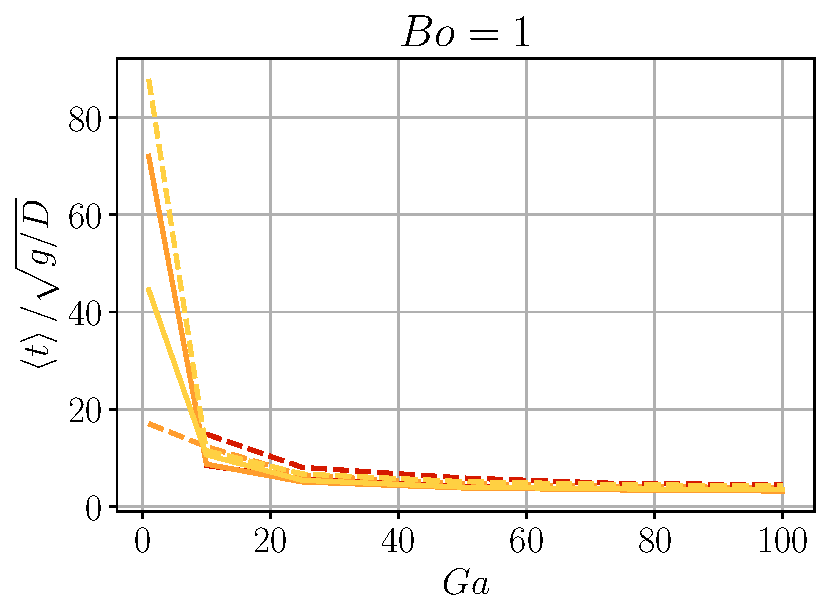
\includegraphics[height=0.20\textheight]{image/N_10/time/Tcm_Bo_1.pdf}
    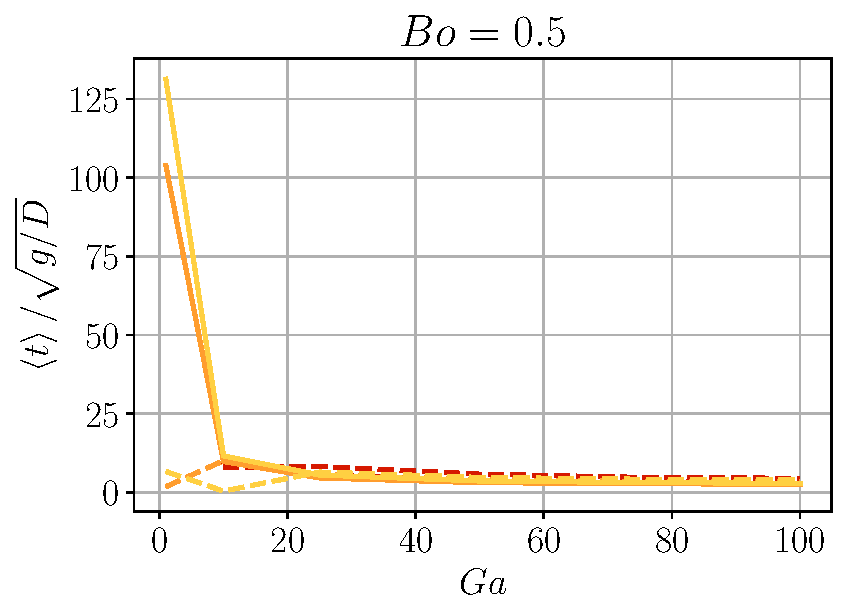
\includegraphics[height=0.20\textheight]{image/N_10/time/Tcm_Bo_0_5.pdf}
    \caption{Averaged dimensionless time of contact. Dashed lines : $\mu_f = 0.42$, solid lines : $\mu_f = 0.042$. \textcolor{red}{\textbf{--}} : $\phi = 0.05$, \textcolor{orange}{\textbf{--}} : $\phi = 0.15$, \textcolor{yellow}{\textbf{--}} : $\phi = 0.25$} 
    \label{fig:time_of_c}
\end{figure} 
\begin{figure}[h!]
    \centering
    \includegraphics[height=0.20\textheight]{image/N_10/freq/HzG_Bo_1.pdf}
    \includegraphics[height=0.20\textheight]{image/N_10/freq/HzG_Bo_0_5.pdf}
    \caption{Dimensionless frequency of contact. Dashed lines : $\mu_f = 0.42$, solid lines : $\mu_f = 0.042$. \textcolor{red}{\textbf{--}} : $\phi = 0.05$, \textcolor{orange}{\textbf{--}} : $\phi = 0.15$, \textcolor{yellow}{\textbf{--}} : $\phi = 0.25$} 
    \label{fig:freq_of_c}
\end{figure} 





\subsubsection*{The 3 dimensional space simulations} 
We are also able to perform 3 dimensional simulations. 
But obviously they take a serious amount of time and resources. 
That is why we preferred to identify the issues and tendency why the 2D cases and launch 3D simulations in a second step. 
Nevertheless, the setup of the 3D cases works fine, and we could already launch some. 
On \ref{fig:3D} we can observe a tri-periodic simulation of 216 buoyant droplets.
Even through the data are not post treated yet the results look very promising. 
\begin{figure}[h!]
    \centering
    \includegraphics[width =  0.7\textwidth]{image/3D/sim49.png}
    \caption{Tri-periodic simulation of 216 drops, $N=7$, $\phi=15$, $Ga = 10$, $Bo =0.5$, the color-map represent the velocity along the $x$ axis. }
    \label{fig:3D}
\end{figure}


\tb{In this limit we observe no coalescence and a homogeneous distribution of particles. 
Therefore, it is possible to derive a theoretical closure model based on periodic green functions.}

\tb{The conclusion is that at very low $Ga$ there is no contact in mono-sized distribution. 
Nevertheless, what would happen for poly-dispersed suspension ?}

\tb{\subsubsection{Poly disperse simulations}}


\subsubsection{Remarks and discussions}
Now let's end this section by pointing out the hardship to come. 
The first major problem is that we have a total of $5$ dimensionless parameters in this study. 
As an example, if we were to carry out one simulation for, let's say, five values per parameters (which would be sufficient to derive empirical laws) it would result in $5^5 = 3125$ simulations. 
While it might be possible in 2D it will surely not be in 3D.
Therefore, in a future work we need to carry out model reduction by using sensibility analysis. 
Furthermore, we encountered another problem by running long time simulations. 
It does seem that the momentum is not well conserved due to the VOF method.
It results in accelerating the bulk, which ultimately reduce the time step du to the CFL condition. 
This problem has already been pointed out by \citet{Naanouh2021numerical} and is already understood. 
The last issue that we could note happens at the limiting cases. 
Indeed, were the parameters are very low / or high some limitations arise. 
For example, when $Bo \rightarrow 0$ the time step reduce dramatically, and when $\phi \rightarrow 0$ (at $N$ constant) the mesh needs a definition that is too expansive (since we need 30 cells per diameter). 